\documentclass[12pt,a4paper]{report}
\pdfminorversion=7

\usepackage[a4paper,margin=1in]{geometry}
\usepackage{mathptmx}
\usepackage{graphicx}
\usepackage{array}
\usepackage{booktabs}
\usepackage{longtable}
\usepackage{multirow}
\usepackage{setspace}
\usepackage{hyperref}
\usepackage{enumitem}
\usepackage{float}
\usepackage{xcolor}
\usepackage{tikz}
\usepackage{pdfpages}
\usepackage{titlesec}

\definecolor{diagNavy}{HTML}{1F3A5F}
\definecolor{diagTeal}{HTML}{2A9D8F}
\definecolor{diagSky}{HTML}{EAF2FB}
\definecolor{diagMint}{HTML}{E8F6F3}
\definecolor{diagSand}{HTML}{FFF5E8}
\definecolor{diagGold}{HTML}{C79A3B}
\definecolor{diagSlate}{HTML}{4A5568}
\definecolor{diagLine}{HTML}{3F4F63}
\definecolor{diagWhite}{HTML}{FFFFFF}

\usetikzlibrary{arrows.meta,positioning,shapes.geometric,shapes.multipart,fit,calc}

\titleformat{\chapter}[display]
  {\centering\bfseries\Large}
  {}
  {0pt}
  {\MakeUppercase}
\titlespacing*{\chapter}{0pt}{0pt}{16pt}

\newif\ifshowacademicborder
\showacademicborderfalse
\newcommand{\EnableAcademicBorder}{\global\showacademicbordertrue}

\AddToHook{shipout/background}{%
  \ifshowacademicborder
    \begin{tikzpicture}[remember picture,overlay]
      \draw[line width=1.0pt]
        ($(current page.north west)+(12mm,-12mm)$)
        rectangle
        ($(current page.south east)+(-12mm,12mm)$);
      \draw[line width=0.55pt]
        ($(current page.north west)+(14mm,-14mm)$)
        rectangle
        ($(current page.south east)+(-14mm,14mm)$);
    \end{tikzpicture}
  \fi
}

\setstretch{1.2}
\setlength{\parindent}{0pt}
\setlength{\parskip}{4pt}
\setlength{\emergencystretch}{3em}
\sloppy

\hypersetup{
  colorlinks=true,
  linkcolor=black,
  urlcolor=black,
  citecolor=black,
  pdftitle={Bharat Finvest Internal Operations Management System},
  pdfauthor={Tejas Sudhakar Kamble}
}

\makeatletter
\def\ps@plain{%
  \let\@mkboth\@gobbletwo
  \let\@oddhead\@empty
  \let\@evenhead\@empty
  \def\@oddfoot{\hfill\thepage}
  \def\@evenfoot{\hfill\thepage}
}
\makeatother

\pagestyle{plain}

\begin{document}

\pagenumbering{gobble}
\thispagestyle{empty}

\begin{tikzpicture}[remember picture,overlay]
  \draw[line width=1.0pt]
    ($(current page.north west)+(12mm,-12mm)$)
    rectangle
    ($(current page.south east)+(-12mm,12mm)$);
  \draw[line width=0.55pt]
    ($(current page.north west)+(14mm,-14mm)$)
    rectangle
    ($(current page.south east)+(-14mm,14mm)$);
\end{tikzpicture}

\begin{center}
\vspace*{0.9cm}
{\Large\bfseries A PROJECT REPORT ON\par}
\vspace{0.9cm}

\setlength{\fboxsep}{12pt}
\setlength{\fboxrule}{1.1pt}
\fbox{\parbox{0.88\textwidth}{
\centering
{\LARGE\bfseries (BHARAT FINVEST INTERNAL OPERATIONS MANAGEMENT SYSTEM)}
}}

\vspace{1.2cm}
{\large\bfseries BY\par}
\vspace{0.3cm}
{\Large\bfseries (TEJAS SUDHAKAR KAMBLE)\par}
\vspace{0.35cm}
{\large M.Sc. (Computer Science) Part II, Sem IV\par}

\vfill
{\large\bfseries INDUSTRIAL TRAINING ORGANIZATION\par}
{\large Nityashree Infosystems Pvt. Ltd.\par}
\vspace{0.5cm}

{\large\bfseries CLIENT DOMAIN ORGANIZATION\par}
{\large Bharat Finvest\par}
\vspace{0.8cm}

{\large Submitted To\par}
{\Large\bfseries SIR PARASHURAMBHAU COLLEGE, PUNE\par}
{\large (2025 -- 2026)\par}
\end{center}

\clearpage
\chapter*{Completion Certificate}
\thispagestyle{empty}
\vspace*{4cm}
\begin{center}
{\Large\bfseries Completion Certificate}\par
\vspace{1.2cm}
\fbox{\parbox{0.85\textwidth}{
\centering
\vspace{1.2cm}
\textit{The company completion certificate from Nityashree Infosystems Pvt. Ltd. will be attached here after official issuance.}
\vspace{1.2cm}
}}
\end{center}
\clearpage

\clearpage

\includepdf[pages=1,fitpaper=true,pagecommand={}]{images/college_certificate_template.pdf}

\clearpage
\EnableAcademicBorder

\pagenumbering{roman}
\setcounter{page}{1}
\chapter*{Declaration}
I, \textbf{Tejas Sudhakar Kamble}, hereby declare that this project report titled \textbf{Bharat Finvest Internal Operations Management System} is my original work carried out as part of the Industrial Training Project for M.Sc. (Computer Science) Part II, Sem IV at Sir Parashurambhau College, Pune.

This project was developed during industrial training at \textbf{Nityashree Infosystems Pvt. Ltd.} as a client-style internal operations management system for \textbf{Bharat Finvest}.

I confirm that:
\begin{itemize}[leftmargin=1.3cm]
\item The work presented in this report has been implemented and validated in the repository \url{https://github.com/tejasskamble/bharat-finvest-ops-system}.
\item The technical descriptions are based on the actual source code, database scripts, and DevOps files present in the project.
\item Wherever external references are used, appropriate acknowledgements are provided.
\end{itemize}

\vspace{1.5cm}
\begin{tabular}{p{8cm}p{6cm}}
Place: Pune & Signature: \rule{3.2cm}{0.4pt} \\
Date: \rule{2.4cm}{0.4pt} & Name: Tejas Sudhakar Kamble
\end{tabular}

\clearpage
\chapter*{Acknowledgement}
I express my sincere gratitude to Sir Parashurambhau College, Pune, Department of Computer Science, for providing the academic platform to complete this Industrial Training Project.

I am thankful to \textbf{Nityashree Infosystems Pvt. Ltd.}, my training organization, for mentorship, professional guidance, and practical exposure during this project period.

\textit{This project was developed during industrial training at Nityashree Infosystems Pvt. Ltd. as a client-style internal operations management system for Bharat Finvest.}

I also acknowledge the operational domain context of \textbf{Bharat Finvest}, which helped shape realistic requirements for employee management, task tracking, attendance, and reporting workflows.

I would like to thank my faculty mentors and evaluators for their continuous guidance throughout requirement analysis, system design, implementation, QA, and documentation stages.

I also acknowledge the support received from peers and colleagues during project discussions, testing reviews, and final quality checks.

Finally, I thank my family for their encouragement and support during the completion of this project.

\clearpage
\chapter*{Abstract}
This report presents the design and implementation of the \textbf{Bharat Finvest Internal Operations Management System}, a full-stack web application developed to digitize core internal workflows such as employee management, task allocation, attendance marking, and operational reporting.

This project was developed during industrial training at \textbf{Nityashree Infosystems Pvt. Ltd.} as a client-style internal operations management system for \textbf{Bharat Finvest}.

The application uses a React + Vite frontend, an Express + Node.js backend, and MySQL as the relational data store. Authentication is implemented through JWT, passwords are secured using bcrypt hashes, and role-based access control is enforced for admin, manager, and employee roles.

The project also includes practical DevOps features such as Dockerized deployment, health checks, GitHub Actions continuous integration, and Windows-based backup/restore scripts. A one-click startup batch file is provided to simplify demonstrations.

The final system provides a reliable dashboard for operational visibility, structured CRUD flows for employees and tasks, attendance analytics, and PDF report export. The implementation reflects a realistic enterprise-style internal portal and is suitable for academic submission as well as live demonstration.

\clearpage
\tableofcontents
\clearpage

\pagenumbering{arabic}
\setcounter{page}{1}
\chapter{Introduction to Problem}

Financial operations teams in many organizations still depend on disconnected tools such as spreadsheets, WhatsApp updates, and manual registers for daily tracking. This creates fragmentation in information flow and delays operational decisions.

This project was developed during industrial training at \textbf{Nityashree Infosystems Pvt. Ltd.} as a client-style internal operations management system for \textbf{Bharat Finvest}.

In the Bharat Finvest client context, the following problem areas were identified:
\begin{itemize}[leftmargin=1.3cm]
\item Employee master data and status were not centrally visible to all stakeholders.
\item Task assignment and progress tracking lacked a single source of truth.
\item Attendance updates required repetitive manual consolidation.
\item Operational reports were time-consuming to prepare and difficult to standardize.
\item Role-specific data access and accountability were difficult to enforce consistently.
\end{itemize}

The project addresses these problems by delivering a web-based internal portal that combines authentication, role-based workflow, operational dashboards, and structured reporting.

The structure and chapter sequence used in this report follow the academic format observed from the provided reference files (cover page style, certificate pattern, index pattern, and internal evaluation guideline sequence).

\chapter{Existing System}

Before implementation, the typical process in similar setups was:
\begin{enumerate}[leftmargin=1.3cm]
\item Employee details were maintained in spreadsheets.
\item Task updates were shared through informal communication.
\item Attendance was maintained through separate logs and periodic manual aggregation.
\item Reporting was generated manually, often by copying data between files.
\end{enumerate}

\textbf{Observed Limitations}
\begin{itemize}[leftmargin=1.3cm]
\item Data duplication and version conflicts.
\item Limited traceability for who changed what and when.
\item No unified role-based interface for admin/manager/employee users.
\item Delayed reporting and inconsistent report formats.
\item Difficult quality assurance due to multiple disconnected sources.
\end{itemize}

The absence of a centralized application directly impacted productivity and operational control.

\chapter{Proposed System}

The proposed solution is a centralized internal operations management portal with secure login and role-aware access.

\textbf{Core goals of the proposed system:}
\begin{itemize}[leftmargin=1.3cm]
\item Single application for employee, task, attendance, and reporting workflows.
\item JWT-based login with backend authorization checks.
\item Dashboard with live operational metrics.
\item CRUD-based data management with validations and error handling.
\item PDF report export for submission and review use cases.
\item DevOps readiness through Docker, CI, health checks, and backup utilities.
\end{itemize}

\textbf{User roles in system:}
\begin{itemize}[leftmargin=1.3cm]
\item \textbf{Admin}: Full access including employee deactivation and task deletion.
\item \textbf{Manager}: Operational management access (employee/task/attendance updates except admin-only actions).
\item \textbf{Employee}: Read-focused access to operational pages as configured by role restrictions.
\end{itemize}

\chapter{Scope of Work}

This project was developed during industrial training at \textbf{Nityashree Infosystems Pvt. Ltd.} as a client-style internal operations management system for \textbf{Bharat Finvest}.

The project scope covered end-to-end lifecycle stages:

\textbf{1. Requirement Understanding}
\begin{itemize}[leftmargin=1.3cm]
\item Identify entities: users, employees, tasks, attendance.
\item Define role behaviors and API-level restrictions.
\item Define reporting requirements and demo credentials.
\end{itemize}

\textbf{2. Application Development}
\begin{itemize}[leftmargin=1.3cm]
\item Frontend implementation with React, Vite, Bootstrap.
\item Backend API implementation with Express and MySQL2.
\item JWT authentication and authorization middleware.
\end{itemize}

\textbf{3. Data Modeling}
\begin{itemize}[leftmargin=1.3cm]
\item Relational schema design for users, employees, tasks, attendance.
\item Seed dataset creation including employee and intern records.
\end{itemize}

\textbf{4. DevOps and Operations}
\begin{itemize}[leftmargin=1.3cm]
\item Docker Compose environment for frontend, backend, and MySQL.
\item Health check API and container health validation.
\item CI pipeline for backend import verification and frontend build.
\item Backup and restore scripts for database operations.
\end{itemize}

\textbf{5. QA and Stabilization}
\begin{itemize}[leftmargin=1.3cm]
\item Validation of all major UI actions and backend responses.
\item Error handling, confirmation prompts, and loading states.
\item Final data consistency verification for demo safety.
\end{itemize}

\textbf{Out of Scope Clarification}
\begin{itemize}[leftmargin=1.3cm]
\item Official production deployment and live organization roll-out are outside the current academic project scope.
\item No claim is made for official production adoption by Bharat Finvest in this report.
\end{itemize}

\chapter{Feasibility Study}

\section{Technical Feasibility}
The required technology stack is mature and widely supported. React, Node.js, Express, and MySQL are stable for CRUD-centric enterprise applications. The project successfully integrates authentication, role middleware, charting, and PDF export.

\section{Operational Feasibility}
The target users (admin, manager, employee) interact through simple forms, tables, and filters. One-click launcher and explicit command documentation reduce operational friction during demos and daily usage.

\section{Economic Feasibility}
The project uses open-source frameworks and tooling. Local setup requires standard development machines and optional Docker Desktop. There is no mandatory paid dependency in the implementation.

\chapter{System Requirements}

\section{Hardware Requirements}
\begin{table}[H]
\centering
\begin{tabular}{p{5cm}p{9cm}}
\toprule
\textbf{Component} & \textbf{Recommended Specification} \\
\midrule
Processor & Intel i5 / AMD Ryzen 5 or higher \\
RAM & Minimum 8 GB (16 GB preferred) \\
Storage & 10 GB free space for code, packages, Docker images \\
Network & Internet required for dependency installation and Git operations \\
\bottomrule
\end{tabular}
\end{table}

\section{Software Requirements}
\begin{table}[H]
\centering
\begin{tabular}{p{5cm}p{9cm}}
\toprule
\textbf{Software} & \textbf{Purpose} \\
\midrule
Windows 10/11 & Development and execution environment \\
Node.js (18+) & Runtime for backend and frontend tooling \\
npm & Package management \\
MySQL 8.0 & Relational database \\
Git & Version control \\
Docker Desktop (optional) & Containerized deployment \\
VS Code & Source code editing \\
\bottomrule
\end{tabular}
\end{table}

\chapter{Technology Stack}

\begin{longtable}{p{3.2cm}p{3.2cm}p{8.0cm}}
\toprule
\textbf{Layer} & \textbf{Technology} & \textbf{Usage in Project} \\
\midrule
\endhead
Frontend & React.js & Component-based UI for login, dashboard, employees, tasks, attendance, and reports pages. \\
Frontend Tooling & Vite & Fast development server and production build pipeline. \\
UI Framework & Bootstrap 5 & Responsive layout, tables, modals, forms, alerts, buttons. \\
HTTP Client & Axios & API requests through centralized axios instance with auth header interceptor. \\
Charts & Chart.js + react-chartjs-2 & Dashboard visualization for task status and attendance. \\
Reporting & jsPDF + jspdf-autotable & Client-side PDF exports for employee/task/attendance reports. \\
Backend Runtime & Node.js & JavaScript runtime for API server. \\
Backend Framework & Express.js & Route handling, middleware, JSON APIs, error responses. \\
Database Driver & mysql2/promise & Parameterized SQL query execution. \\
Database & MySQL 8.0 & Persistent storage for users, employees, tasks, attendance. \\
Authentication & JWT & Stateless token authentication with Bearer headers. \\
Password Security & bcrypt & Secure password hash verification during login. \\
DevOps & Docker, Docker Compose & Multi-service orchestration: mysql, backend, frontend. \\
CI/CD & GitHub Actions & Automated dependency install, backend import check, frontend build. \\
\bottomrule
\end{longtable}

\chapter{System Architecture}

The implemented system follows a three-tier architecture with an additional DevOps support layer.

\begin{itemize}[leftmargin=1.3cm]
\item \textbf{Presentation Layer}: React + Vite frontend, served in development at port 5173 and through Nginx in Docker.
\item \textbf{Application Layer}: Express backend at port 5000, exposing REST APIs under \texttt{/api/*}.
\item \textbf{Data Layer}: MySQL database with normalized relational schema.
\item \textbf{DevOps Layer}: Docker Compose orchestration, health checks, GitHub Actions CI, backup/restore scripts.
\end{itemize}

\begin{figure}[H]
\centering
\resizebox{0.95\textwidth}{!}{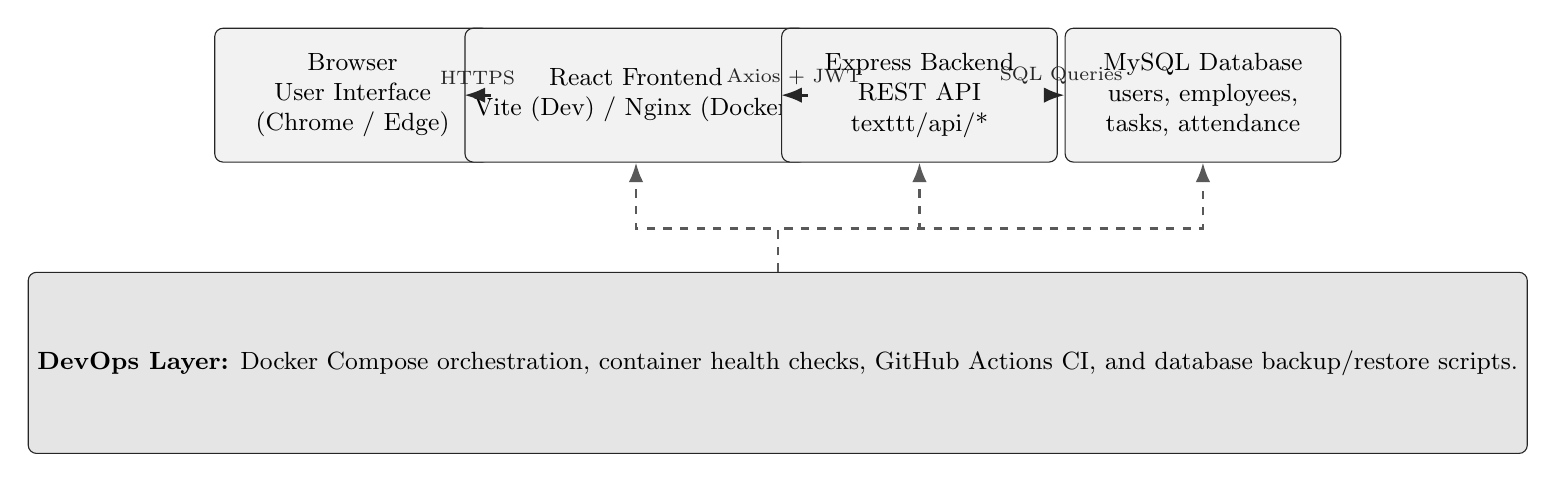
\begin{tikzpicture}[
  font=\small,
  >=Latex,
  layerbox/.style={draw=black!85, rounded corners=3pt, fill=black!5, minimum width=3.5cm, minimum height=1.7cm, align=center},
  devops/.style={draw=black!85, rounded corners=3pt, fill=black!10, minimum width=14.4cm, minimum height=2.3cm, align=left},
  flow/.style={-Latex, line width=1.0pt, black!85},
  support/.style={-Latex, line width=0.9pt, black!65, dashed}
]

\node[layerbox] (browser) at (-5.4,1.8) {Browser\\User Interface\\(Chrome / Edge)};
\node[layerbox] (frontend) at (-1.8,1.8) {React Frontend\\Vite (Dev) / Nginx (Docker)};
\node[layerbox] (backend) at (1.8,1.8) {Express Backend\\REST API \\texttt{/api/*}};
\node[layerbox] (database) at (5.4,1.8) {MySQL Database\\users, employees,\\tasks, attendance};

\draw[flow] (browser.east) -- node[above, font=\scriptsize] {HTTPS} (frontend.west);
\draw[flow] (frontend.east) -- node[above, font=\scriptsize] {Axios + JWT} (backend.west);
\draw[flow] (backend.east) -- node[above, font=\scriptsize] {SQL Queries} (database.west);

\node[devops] (ops) at (0,-1.6) {\textbf{DevOps Layer:} Docker Compose orchestration, container health checks, GitHub Actions CI, and database backup/restore scripts.};

\draw[support] (ops.north) -- ++(0,0.55) -| (frontend.south);
\draw[support] (ops.north) -- ++(0,0.55) -| (backend.south);
\draw[support] (ops.north) -- ++(0,0.55) -| (database.south);

\end{tikzpicture}
}
\caption{System Architecture Diagram}
\end{figure}

\textbf{Request Flow Summary}
\begin{enumerate}[leftmargin=1.3cm]
\item User action in frontend triggers an Axios request.
\item Axios interceptor attaches JWT token (if present).
\item Backend middleware verifies token and role.
\item Controller executes parameterized SQL on MySQL.
\item JSON response updates UI state and renders feedback.
\end{enumerate}

\chapter{Database Design}

The database schema is defined in \texttt{database/schema.sql} and seeded through \texttt{database/seed.sql}.

\section{Tables}
\subsection*{1. users}
Stores authenticated application users.
\begin{itemize}[leftmargin=1.3cm]
\item Primary Key: \texttt{id}
\item Key fields: \texttt{name}, \texttt{email} (unique), \texttt{password\_hash}, \texttt{role}, \texttt{department}
\item Role values: \texttt{admin}, \texttt{manager}, \texttt{employee}
\end{itemize}

\subsection*{2. employees}
Stores employee and intern profile records.
\begin{itemize}[leftmargin=1.3cm]
\item Primary Key: \texttt{id}
\item Foreign Key: \texttt{user\_id} references \texttt{users(id)}
\item Unique field: \texttt{employee\_code}
\item Key fields: \texttt{name}, \texttt{email}, \texttt{phone}, \texttt{department}, \texttt{designation}, \texttt{date\_of\_joining}, \texttt{status}
\item Status values: \texttt{active}, \texttt{inactive}
\end{itemize}

\subsection*{3. tasks}
Stores tasks assigned to employees.
\begin{itemize}[leftmargin=1.3cm]
\item Primary Key: \texttt{id}
\item Foreign Keys: \texttt{assigned\_to} references \texttt{employees(id)}, \texttt{assigned\_by} references \texttt{users(id)}
\item Key fields: \texttt{title}, \texttt{description}, \texttt{priority}, \texttt{status}, \texttt{due\_date}
\item Priority values: \texttt{low}, \texttt{medium}, \texttt{high}
\item Status values: \texttt{pending}, \texttt{in\_progress}, \texttt{completed}
\end{itemize}

\subsection*{4. attendance}
Stores attendance logs per employee and date.
\begin{itemize}[leftmargin=1.3cm]
\item Primary Key: \texttt{id}
\item Foreign Key: \texttt{employee\_id} references \texttt{employees(id)}
\item Unique composite key: \texttt{(employee\_id, date)}
\item Status values: \texttt{present}, \texttt{absent}, \texttt{half\_day}, \texttt{leave}
\end{itemize}

\section{Relationship Notes}
\begin{itemize}[leftmargin=1.3cm]
\item One user may be linked to zero or one employee profile (\texttt{users} to \texttt{employees}).
\item One employee can have many tasks and many attendance records.
\item One admin/manager user can assign many tasks.
\item Cascade operations are handled carefully in APIs to avoid accidental data deletion in demo scenarios.
\end{itemize}

\section{Seed Data Highlights}
\begin{itemize}[leftmargin=1.3cm]
\item Demo users: Admin (Akshay Shinde), Manager (Pravin Shinde), Employee (Ritesh Bhate).
\item Employee table includes 8 regular employees and 4 interns (total 12 records).
\item Seed includes realistic tasks and attendance records for reporting and dashboard visualization.
\end{itemize}

\chapter{ER Diagram}

The following ER diagram represents the relational model used in the current project.

\begin{figure}[H]
\centering
\resizebox{0.95\textwidth}{!}{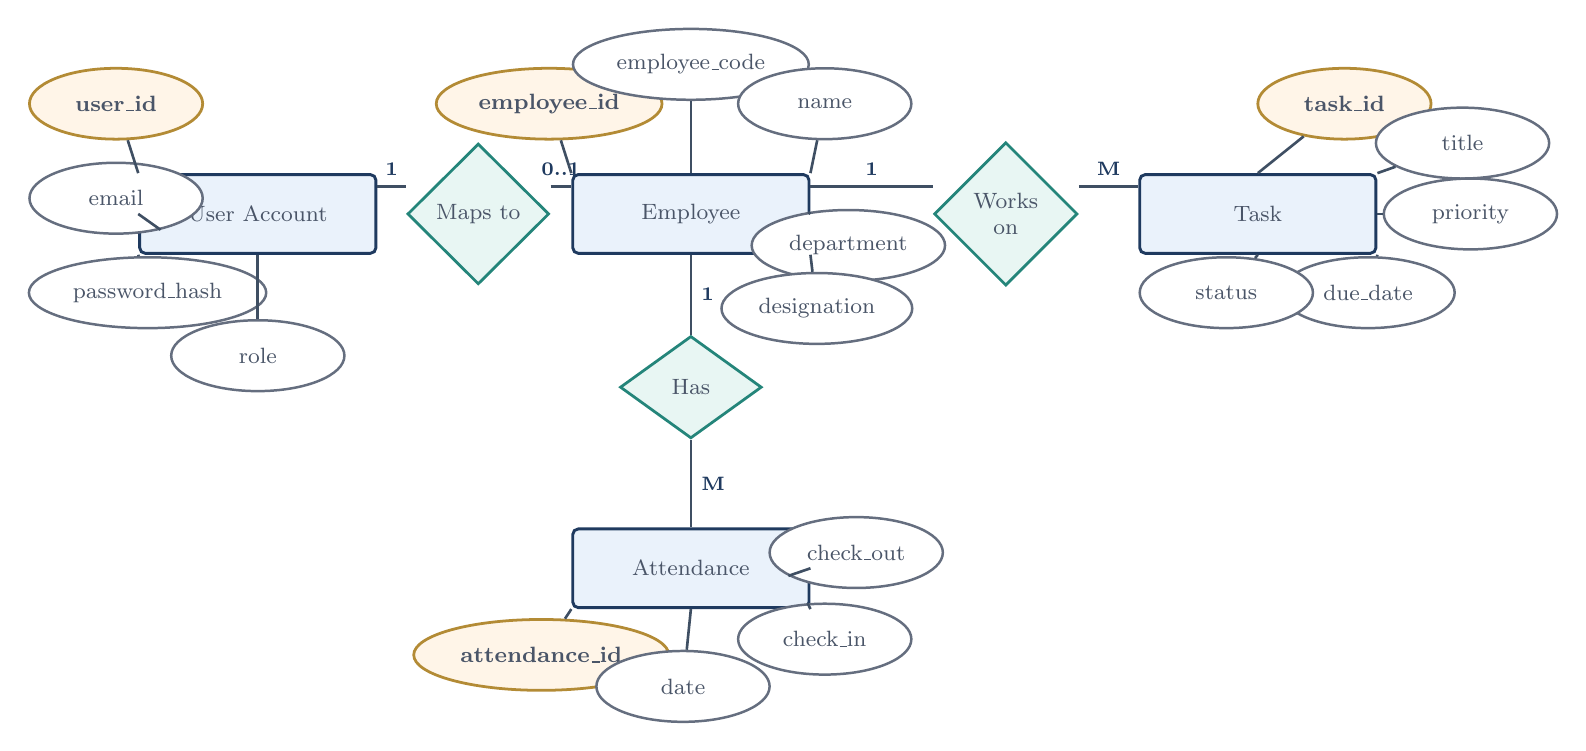
\begin{tikzpicture}[
  font=\footnotesize,
  entity/.style={draw=diagNavy, line width=1.05pt, rounded corners=2pt, minimum width=3.0cm, minimum height=1.0cm, fill=diagSky, align=center, text=diagSlate},
  attr/.style={ellipse, draw=diagSlate!85, line width=0.9pt, minimum width=2.2cm, minimum height=0.9cm, fill=diagWhite, align=center, text=diagSlate},
  keyattr/.style={attr, draw=diagGold!90!black, fill=diagSand, line width=1.0pt, font=\footnotesize\bfseries},
  relation/.style={diamond, draw=diagTeal!85!black, line width=1.0pt, minimum width=1.8cm, minimum height=1.3cm, fill=diagMint, align=center, text=diagSlate},
  link/.style={line width=0.95pt, diagLine},
  card/.style={font=\scriptsize\bfseries, text=diagNavy}
]

% Entities
\node[entity] (users) at (-7.0,1.4) {User Account};
\node[entity] (employees) at (-1.5,1.4) {Employee};
\node[entity] (tasks) at (5.7,1.4) {Task};
\node[entity] (attendance) at (-1.5,-3.1) {Attendance};

% Relationships
\node[relation] (mapsTo) at (-4.2,1.4) {Maps to};
\node[relation] (worksOn) at (2.5,1.4) {Works\\on};
\node[relation] (has) at (-1.5,-0.8) {Has};

% Relationship links + cardinalities
\draw[link] ([yshift=10pt]users.east) -- ([yshift=10pt]mapsTo.west) node[midway, above, card] {1};
\draw[link] ([yshift=10pt]mapsTo.east) -- ([yshift=10pt]employees.west) node[midway, above, card] {0..1};
\draw[link] ([yshift=10pt]employees.east) -- ([yshift=10pt]worksOn.west) node[midway, above, card] {1};
\draw[link] ([yshift=10pt]worksOn.east) -- ([yshift=10pt]tasks.west) node[midway, above, card] {M};
\draw[link] (employees.south) -- (has.north) node[midway, right, card] {1};
\draw[link] (has.south) -- (attendance.north) node[midway, right, card] {M};

% User attributes
\node[keyattr] (userId) at (-8.8,2.8) {user\_id};
\node[attr] (uEmail) at (-8.8,1.6) {email};
\node[attr] (uPass) at (-8.4,0.4) {password\_hash};
\node[attr] (uRole) at (-7.0,-0.4) {role};
\draw[link] (userId) -- (users.north west);
\draw[link] (uEmail) -- (users.west);
\draw[link] (uPass) -- (users.south west);
\draw[link] (uRole) -- (users.south);

% Employee attributes
\node[keyattr] (empId) at (-3.3,2.8) {employee\_id};
\node[attr] (empCode) at (-1.5,3.3) {employee\_code};
\node[attr] (empName) at (0.2,2.8) {name};
\node[attr] (empDept) at (0.5,1.0) {department};
\node[attr] (empDesig) at (0.1,0.2) {designation};
\draw[link] (empId) -- (employees.north west);
\draw[link] (empCode) -- (employees.north);
\draw[link] (empName) -- (employees.north east);
\draw[link] (empDept) -- (employees.east);
\draw[link] (empDesig) -- (employees.south east);

% Task attributes
\node[keyattr] (taskId) at (6.8,2.8) {task\_id};
\node[attr] (tTitle) at (8.3,2.3) {title};
\node[attr] (tPriority) at (8.4,1.4) {priority};
\node[attr] (tDue) at (7.1,0.4) {due\_date};
\node[attr] (tStatus) at (5.3,0.4) {status};
\draw[link] (taskId) -- (tasks.north);
\draw[link] (tTitle) -- (tasks.north east);
\draw[link] (tPriority) -- (tasks.east);
\draw[link] (tDue) -- (tasks.south east);
\draw[link] (tStatus) -- (tasks.south);

% Attendance attributes
\node[keyattr] (attId) at (-3.4,-4.2) {attendance\_id};
\node[attr] (aDate) at (-1.6,-4.6) {date};
\node[attr] (aIn) at (0.2,-4.0) {check\_in};
\node[attr] (aOut) at (0.6,-2.9) {check\_out};
\draw[link] (attId) -- (attendance.south west);
\draw[link] (aDate) -- (attendance.south);
\draw[link] (aIn) -- (attendance.south east);
\draw[link] (aOut) -- (attendance.east);

\end{tikzpicture}
}
\caption{Entity Relationship Diagram}
\end{figure}

\chapter{UML Diagrams}

The UML diagrams used to represent the system design are as follows:
\begin{itemize}[leftmargin=1.4cm]
  \item Activity Diagram
  \item Use Case Diagram
  \item Class Diagram
  \item Sequence Diagram
\end{itemize}

\section{Activity Diagram}
\begin{figure}[H]
\centering
\resizebox{0.90\textwidth}{!}{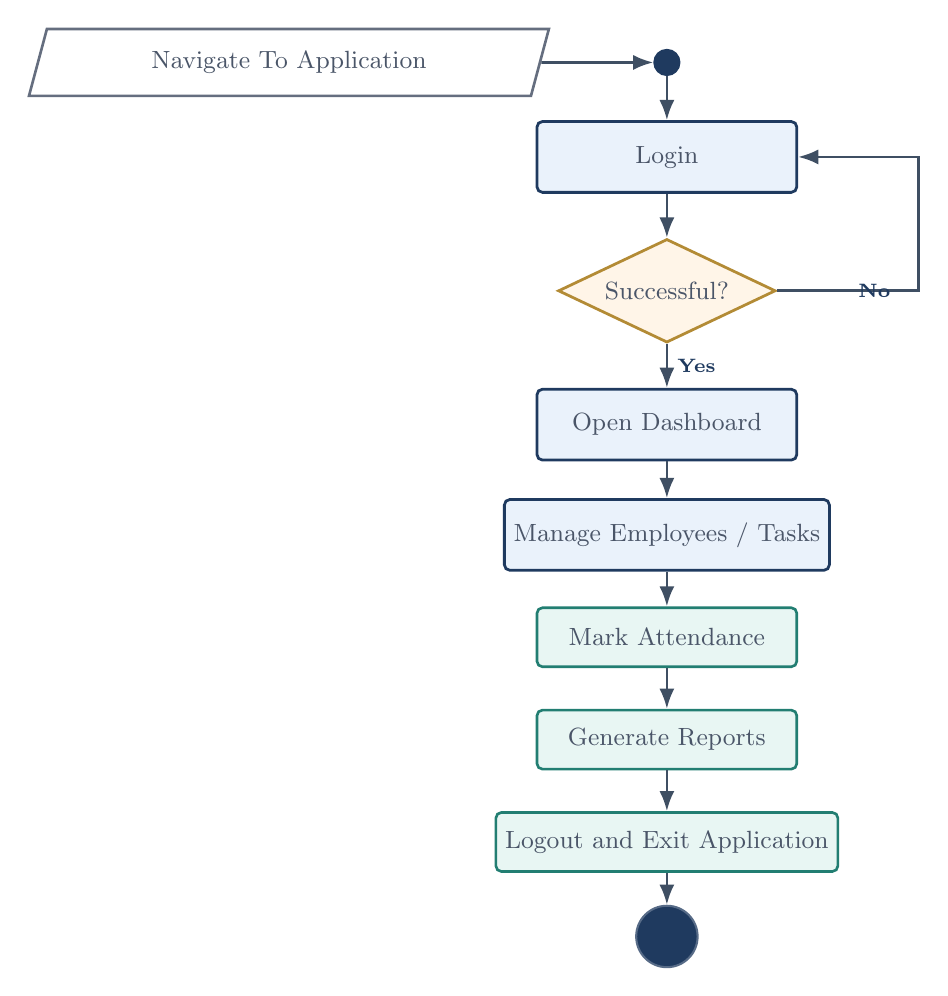
\begin{tikzpicture}[
  font=\small,
  >=Latex,
  action/.style={draw=diagNavy, line width=1.0pt, rounded corners=2pt, minimum width=3.3cm, minimum height=0.9cm, align=center, fill=diagSky, text=diagSlate},
  substep/.style={draw=diagTeal!80!black, line width=0.95pt, rounded corners=2pt, minimum width=3.3cm, minimum height=0.75cm, align=center, fill=diagMint, text=diagSlate},
  decision/.style={draw=diagGold!90!black, line width=1.0pt, diamond, aspect=2.1, minimum width=2.2cm, minimum height=1.0cm, align=center, fill=diagSand, text=diagSlate},
  flow/.style={-Latex, line width=0.95pt, diagLine},
  label/.style={font=\scriptsize\bfseries, text=diagNavy}
]

% Initial and final states
\node[circle, draw=diagNavy, fill=diagNavy, minimum size=0.28cm] (start) at (1.6,6.0) {};
\node[circle, draw=diagNavy!75, line width=0.75pt, fill=diagNavy, minimum size=0.78cm] (end) at (1.6,-5.1) {};

% Top navigation action (left to right)
\node[draw=diagSlate!85, line width=0.95pt, trapezium, trapezium left angle=75, trapezium right angle=105, minimum width=4.2cm, minimum height=0.85cm, fill=diagWhite, text=diagSlate] (nav) at (-3.2,6.0) {Navigate To Application};
\draw[flow] (nav.east) -- (start.west);

% Main flow
\node[action] (login) at (1.6,4.8) {Login};
\node[decision] (valid) at (1.6,3.1) {Successful?};
\node[action] (dashboard) at (1.6,1.4) {Open Dashboard};
\node[action] (manage) at (1.6,0.0) {Manage Employees / Tasks};
\node[substep] (attendance) at (1.6,-1.3) {Mark Attendance};
\node[substep] (reports) at (1.6,-2.6) {Generate Reports};
\node[substep] (logout) at (1.6,-3.9) {Logout and Exit Application};

\draw[flow] (start) -- (login);
\draw[flow] (login) -- (valid);
\draw[flow] (valid) -- node[right, label] {Yes} (dashboard);
\draw[flow] (dashboard) -- (manage);
\draw[flow] (manage) -- (attendance);
\draw[flow] (attendance) -- (reports);
\draw[flow] (reports) -- (logout);
\draw[flow] (logout) -- (end);

% No branch loops back to login
\draw[flow] (valid.east) -- ++(1.8,0) node[midway, right, label] {No} -- ++(0,1.7) -- (login.east);

\end{tikzpicture}
}
\caption{Activity Diagram}
\end{figure}
\clearpage

\section{Use Case Diagram}
\begin{figure}[H]
\centering
\resizebox{0.95\textwidth}{!}{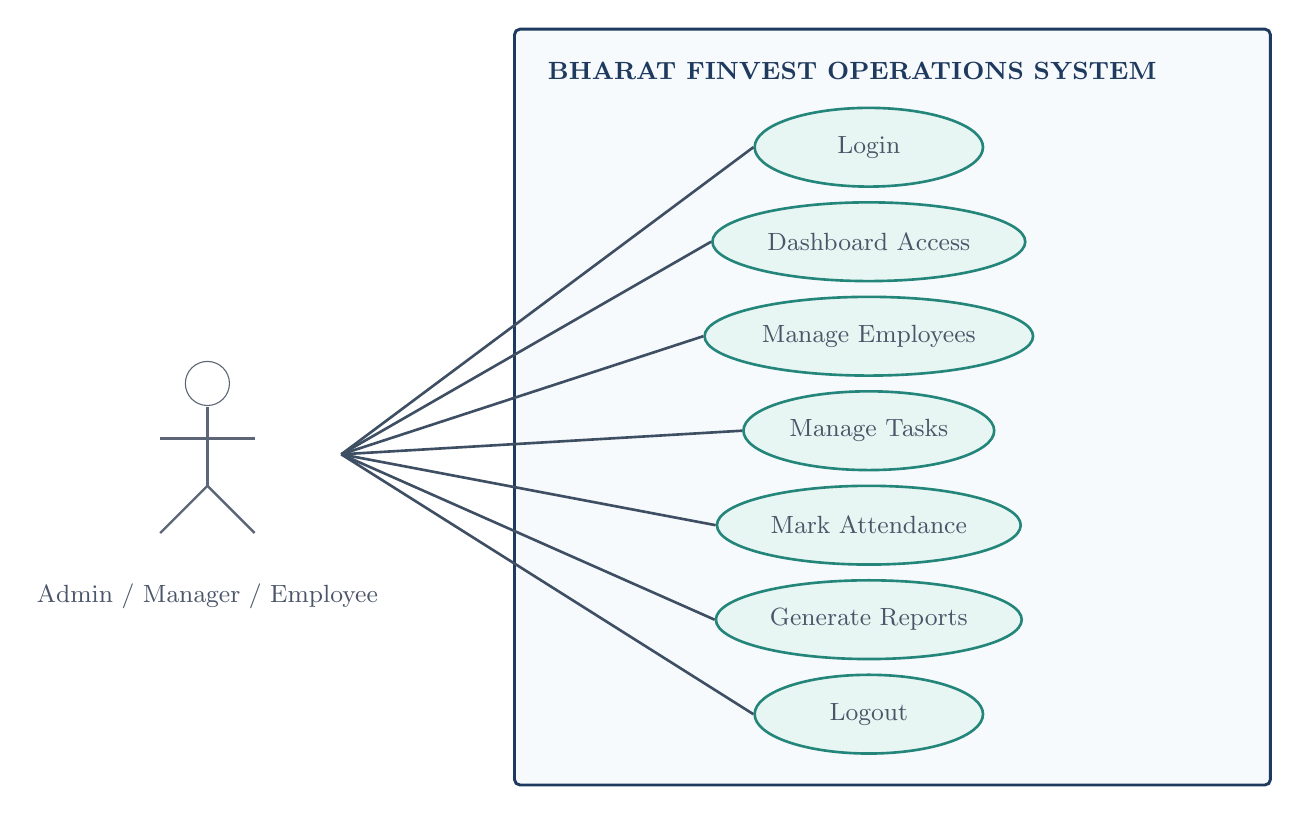
\begin{tikzpicture}[
  font=\small,
  usecase/.style={draw=diagTeal!85!black, line width=0.95pt, ellipse, minimum width=2.9cm, minimum height=1.0cm, fill=diagMint, align=center, text=diagSlate},
  assoc/.style={line width=0.95pt, diagLine}
]

% System boundary
\node[draw=diagNavy, line width=1.05pt, rounded corners=2pt, minimum width=9.6cm, minimum height=9.6cm, fill=diagSky!40] (system) at (2.8,-0.4) {};
\node[anchor=north west, font=\small\bfseries, text=diagNavy] at (-1.7,4.1) {BHARAT FINVEST OPERATIONS SYSTEM};

% Actor (stick figure)
\coordinate (head) at (-5.9,-0.1);
\draw[diagSlate!90] (head) circle (0.28cm);
\draw[diagSlate!90, line width=0.85pt] (-5.9,-0.4) -- (-5.9,-1.4);
\draw[diagSlate!90, line width=0.85pt] (-6.5,-0.8) -- (-5.3,-0.8);
\draw[diagSlate!90, line width=0.85pt] (-5.9,-1.4) -- (-6.5,-2.0);
\draw[diagSlate!90, line width=0.85pt] (-5.9,-1.4) -- (-5.3,-2.0);
\node[align=center, text=diagSlate] at (-5.9,-2.8) {Admin / Manager / Employee};

% Use cases (vertical as per sample structure)
\node[usecase] (login) at (2.5,2.9) {Login};
\node[usecase] (dashboard) at (2.5,1.7) {Dashboard Access};
\node[usecase] (emp) at (2.5,0.5) {Manage Employees};
\node[usecase] (tasks) at (2.5,-0.7) {Manage Tasks};
\node[usecase] (attendance) at (2.5,-1.9) {Mark Attendance};
\node[usecase] (reports) at (2.5,-3.1) {Generate Reports};
\node[usecase] (logout) at (2.5,-4.3) {Logout};

% Fan-out connection hub
\coordinate (hub) at (-4.2,-1.0);
\draw[assoc] (hub) -- (login.west);
\draw[assoc] (hub) -- (dashboard.west);
\draw[assoc] (hub) -- (emp.west);
\draw[assoc] (hub) -- (tasks.west);
\draw[assoc] (hub) -- (attendance.west);
\draw[assoc] (hub) -- (reports.west);
\draw[assoc] (hub) -- (logout.west);

\end{tikzpicture}
}
\caption{Use Case Diagram}
\end{figure}
\clearpage

\section{Class Diagram}
\begin{figure}[H]
\centering
\resizebox{0.95\textwidth}{!}{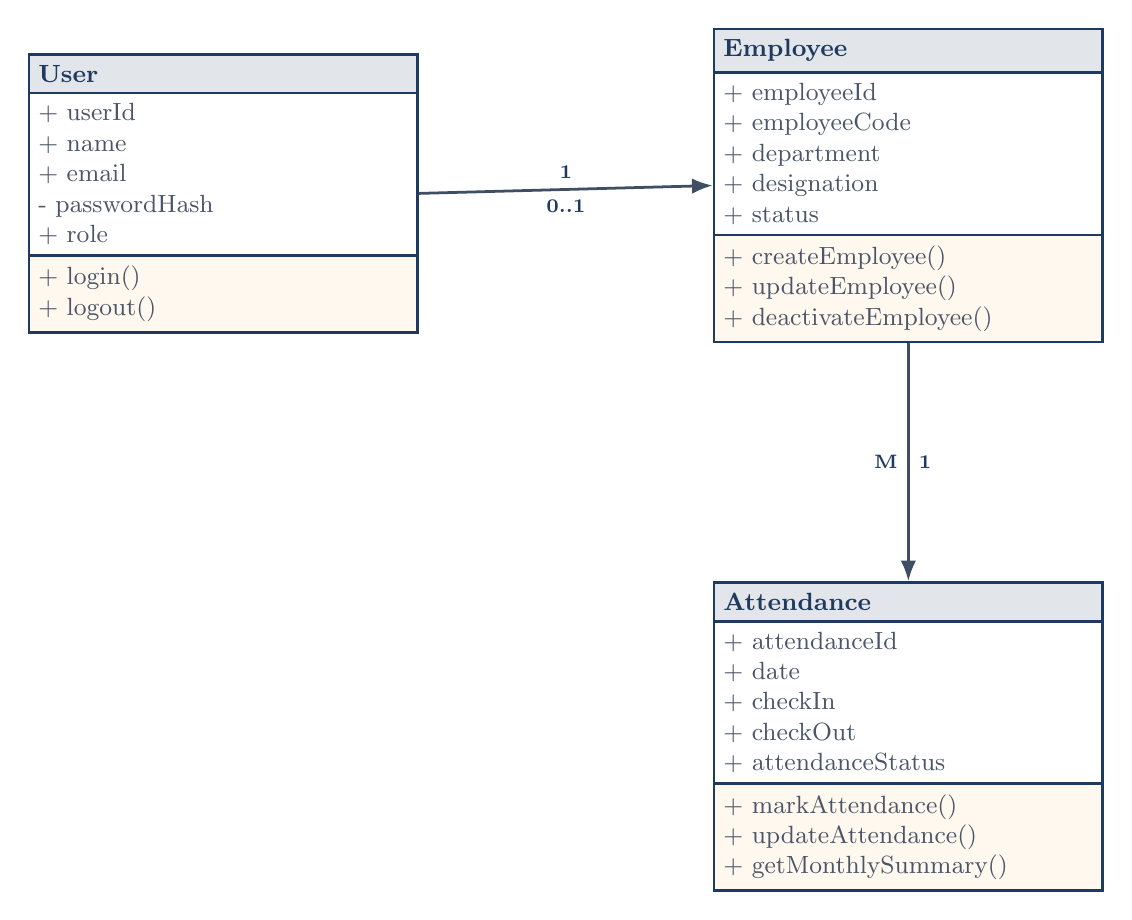
\begin{tikzpicture}[
  font=\small,
  >=Latex,
  classbox/.style={
    draw=diagNavy,
    line width=1.0pt,
    rectangle split,
    rectangle split parts=3,
    rectangle split part align={left,left,left},
    rectangle split part fill={diagNavy!13,diagWhite,diagSand!72},
    text width=4.7cm,
    align=left,
    text=diagSlate
  },
  relation/.style={-Latex, line width=1.0pt, diagLine},
  card/.style={font=\scriptsize\bfseries, text=diagNavy}
]

\node[classbox] (user) at (-5.8,1.8)
{\textcolor{diagNavy}{\textbf{User}}
\nodepart{two}
+ userId\\
+ name\\
+ email\\
- passwordHash\\
+ role
\nodepart{three}
+ login()\\
+ logout()};

\node[classbox] (employee) at (2.9,1.9)
{\textcolor{diagNavy}{\textbf{Employee}}
\nodepart{two}
+ employeeId\\
+ employeeCode\\
+ department\\
+ designation\\
+ status
\nodepart{three}
+ createEmployee()\\
+ updateEmployee()\\
+ deactivateEmployee()};

\node[classbox] (attendance) at (2.9,-5.1)
{\textcolor{diagNavy}{\textbf{Attendance}}
\nodepart{two}
+ attendanceId\\
+ date\\
+ checkIn\\
+ checkOut\\
+ attendanceStatus
\nodepart{three}
+ markAttendance()\\
+ updateAttendance()\\
+ getMonthlySummary()};

% Relations
\draw[relation] (user.east) -- node[above, card] {1} node[below, card] {0..1} (employee.west);
\draw[relation] (employee.south) -- node[right, card] {1} node[left, card] {M} (attendance.north);

\end{tikzpicture}
}
\caption{Class Diagram}
\end{figure}
\clearpage

\section{Sequence Diagram}
\begin{figure}[H]
\centering
\resizebox{0.95\textwidth}{!}{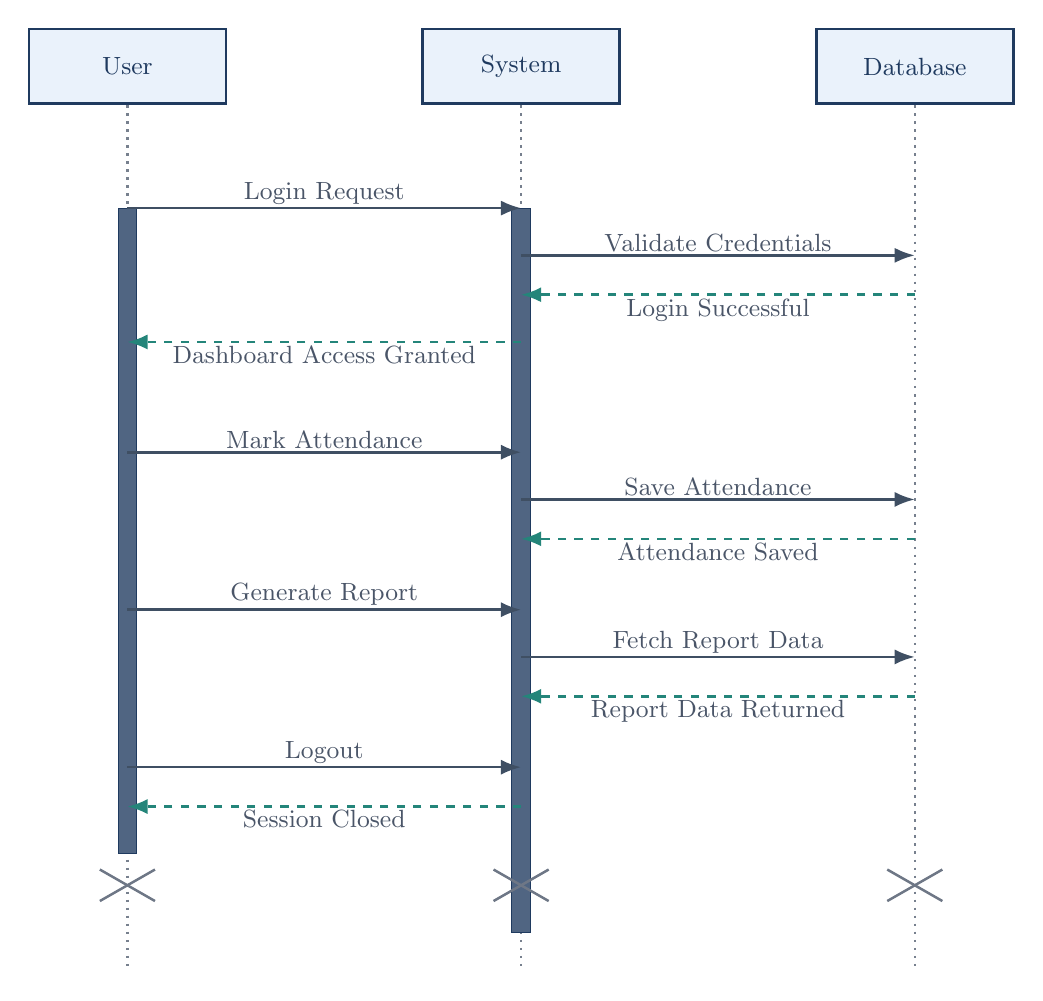
\begin{tikzpicture}[
  font=\small,
  >=Latex,
  participant/.style={draw=diagNavy, line width=0.95pt, fill=diagSky, minimum width=2.5cm, minimum height=0.95cm, align=center, text=diagNavy},
  life/.style={diagSlate!75, dotted, line width=0.9pt},
  activation/.style={draw=diagNavy, fill=diagNavy!78, minimum width=0.14cm},
  call/.style={-Latex, line width=0.95pt, diagLine},
  ret/.style={-Latex, line width=0.95pt, diagTeal!85!black, dashed},
  msglabel/.style={fill=diagWhite, inner sep=1pt, text=diagSlate}
]

% Participants
\node[participant] (actor) at (-5.0,3.9) {User};
\node[participant] (system) at (0.0,3.9) {System};
\node[participant] (db) at (5.0,3.9) {Database};

% Lifelines
\draw[life] (actor.south) -- ++(0,-11.0);
\draw[life] (system.south) -- ++(0,-11.0);
\draw[life] (db.south) -- ++(0,-11.0);

% Activation bars
\node[activation, minimum height=8.2cm] at (-5.0,-2.0) {};
\node[activation, minimum height=9.2cm] at (0.0,-2.5) {};

% Login flow
\draw[call] (-5.0,2.1) -- node[msglabel, above] {Login Request} (0.0,2.1);
\draw[call] (0.0,1.5) -- node[msglabel, above] {Validate Credentials} (5.0,1.5);
\draw[ret] (5.0,1.0) -- node[msglabel, below] {Login Successful} (0.0,1.0);
\draw[ret] (0.0,0.4) -- node[msglabel, below] {Dashboard Access Granted} (-5.0,0.4);

% Attendance flow
\draw[call] (-5.0,-1.0) -- node[msglabel, above] {Mark Attendance} (0.0,-1.0);
\draw[call] (0.0,-1.6) -- node[msglabel, above] {Save Attendance} (5.0,-1.6);
\draw[ret] (5.0,-2.1) -- node[msglabel, below] {Attendance Saved} (0.0,-2.1);

% Reporting flow
\draw[call] (-5.0,-3.0) -- node[msglabel, above] {Generate Report} (0.0,-3.0);
\draw[call] (0.0,-3.6) -- node[msglabel, above] {Fetch Report Data} (5.0,-3.6);
\draw[ret] (5.0,-4.1) -- node[msglabel, below] {Report Data Returned} (0.0,-4.1);

% Logout flow
\draw[call] (-5.0,-5.0) -- node[msglabel, above] {Logout} (0.0,-5.0);
\draw[ret] (0.0,-5.5) -- node[msglabel, below] {Session Closed} (-5.0,-5.5);

% End marks
\draw[diagSlate!80, line width=0.9pt] (-5.35,-6.7) -- (-4.65,-6.3);
\draw[diagSlate!80, line width=0.9pt] (-5.35,-6.3) -- (-4.65,-6.7);
\draw[diagSlate!80, line width=0.9pt] (-0.35,-6.7) -- (0.35,-6.3);
\draw[diagSlate!80, line width=0.9pt] (-0.35,-6.3) -- (0.35,-6.7);
\draw[diagSlate!80, line width=0.9pt] (4.65,-6.7) -- (5.35,-6.3);
\draw[diagSlate!80, line width=0.9pt] (4.65,-6.3) -- (5.35,-6.7);

\end{tikzpicture}
}
\caption{Sequence Diagram}
\end{figure}

\chapter{Module Description}

\section{Login Module}
\textbf{What it does:} Authenticates user credentials and initializes secure session state.

\textbf{Frontend files:}
\begin{itemize}[leftmargin=1.3cm]
\item \texttt{frontend/src/pages/Login.jsx}
\item \texttt{frontend/src/context/AuthContext.jsx}
\item \texttt{frontend/src/api/axiosInstance.js}
\end{itemize}

\textbf{Backend APIs involved:}
\begin{itemize}[leftmargin=1.3cm]
\item \texttt{POST /api/auth/login}
\item \texttt{GET /api/auth/me}
\end{itemize}

\textbf{Database tables:} \texttt{users}

\textbf{Role usage:} Admin, Manager, and Employee.

\section{Admin Dashboard Module}
\textbf{What it does:} Displays operational KPIs and charts such as employee count, task status distribution, and today's attendance summary.

\textbf{Frontend files:}
\begin{itemize}[leftmargin=1.3cm]
\item \texttt{frontend/src/pages/Dashboard.jsx}
\item \texttt{frontend/src/components/StatCard.jsx}
\end{itemize}

\textbf{Backend API involved:} \texttt{GET /api/dashboard/stats}

\textbf{Database tables:} \texttt{employees}, \texttt{tasks}, \texttt{attendance}

\section{Employee Management Module}
\textbf{What it does:} Provides employee search, pagination, add, edit, and activate/deactivate operations.

\textbf{Frontend files:}
\begin{itemize}[leftmargin=1.3cm]
\item \texttt{frontend/src/pages/Employees.jsx}
\item \texttt{frontend/src/components/Avatar.jsx}
\end{itemize}

\textbf{Backend APIs involved:}
\begin{itemize}[leftmargin=1.3cm]
\item \texttt{GET /api/employees}
\item \texttt{GET /api/employees/:id}
\item \texttt{POST /api/employees}
\item \texttt{PUT /api/employees/:id}
\item \texttt{DELETE /api/employees/:id}
\end{itemize}

\textbf{Database tables:} \texttt{employees}, optionally linked to \texttt{users} through \texttt{user\_id}

\textbf{Role behavior:}
\begin{itemize}[leftmargin=1.3cm]
\item Admin and Manager can add/edit employees.
\item Only Admin can deactivate/reactivate employees.
\end{itemize}

\section{Task Management Module}
\textbf{What it does:} Supports task creation, update, filtering by status/priority, and deletion.

\textbf{Frontend files:}
\begin{itemize}[leftmargin=1.3cm]
\item \texttt{frontend/src/pages/Tasks.jsx}
\end{itemize}

\textbf{Backend APIs involved:}
\begin{itemize}[leftmargin=1.3cm]
\item \texttt{GET /api/tasks}
\item \texttt{GET /api/tasks/stats}
\item \texttt{GET /api/tasks/:id}
\item \texttt{POST /api/tasks}
\item \texttt{PUT /api/tasks/:id}
\item \texttt{DELETE /api/tasks/:id}
\end{itemize}

\textbf{Database tables:} \texttt{tasks}, \texttt{employees}, \texttt{users}

\section{Attendance Management Module}
\textbf{What it does:} Tracks daily attendance with filtering and monthly summary.

\textbf{Frontend files:}
\begin{itemize}[leftmargin=1.3cm]
\item \texttt{frontend/src/pages/Attendance.jsx}
\end{itemize}

\textbf{Backend APIs involved:}
\begin{itemize}[leftmargin=1.3cm]
\item \texttt{GET /api/attendance}
\item \texttt{POST /api/attendance}
\item \texttt{PUT /api/attendance/:id}
\item \texttt{GET /api/attendance/summary}
\end{itemize}

\textbf{Database tables:} \texttt{attendance}, \texttt{employees}

\section{Reports Module}
\textbf{What it does:} Generates PDF reports for employees, tasks, and attendance summary using client-side export.

\textbf{Frontend files:}
\begin{itemize}[leftmargin=1.3cm]
\item \texttt{frontend/src/pages/Reports.jsx}
\end{itemize}

\textbf{Backend APIs involved:}
\begin{itemize}[leftmargin=1.3cm]
\item \texttt{GET /api/employees}
\item \texttt{GET /api/tasks}
\item \texttt{GET /api/attendance/summary}
\end{itemize}

\textbf{Libraries:} \texttt{jspdf}, \texttt{jspdf-autotable}

\section{Profile, Branding, and Avatar Module}
\textbf{What it does:} Provides consistent visual identity and dynamic initials-based avatars.

\textbf{Frontend files:}
\begin{itemize}[leftmargin=1.3cm]
\item \texttt{frontend/src/components/Avatar.jsx}
\item \texttt{frontend/src/components/BrandLogo.jsx}
\item \texttt{frontend/src/components/Sidebar.jsx}
\end{itemize}

\textbf{Highlights:}
\begin{itemize}[leftmargin=1.3cm]
\item Removes dependency on static default avatar image for all users.
\item Generates initials from real names (for example, RB, NY, PS, KD).
\item Uses text-based safe branding when official logo asset is unavailable.
\end{itemize}

\section{DevOps Module}
\textbf{What it does:} Standardizes run, verification, health monitoring, CI, and data safety operations.

\textbf{Files:}
\begin{itemize}[leftmargin=1.3cm]
\item \texttt{docker-compose.yml}
\item \texttt{backend/Dockerfile}
\item \texttt{frontend/Dockerfile}
\item \texttt{frontend/nginx.conf}
\item \texttt{.github/workflows/ci.yml}
\item \texttt{scripts/backup-db.bat}
\item \texttt{scripts/restore-db.bat}
\item \texttt{start-project.bat}
\end{itemize}

\textbf{API:} \texttt{GET /api/health}

\chapter{User Interface Screens}

This section documents the primary user interface screens captured from the implemented Bharat Finvest Operations Portal.

\section{Login Screen}
\begin{figure}[H]
\centering
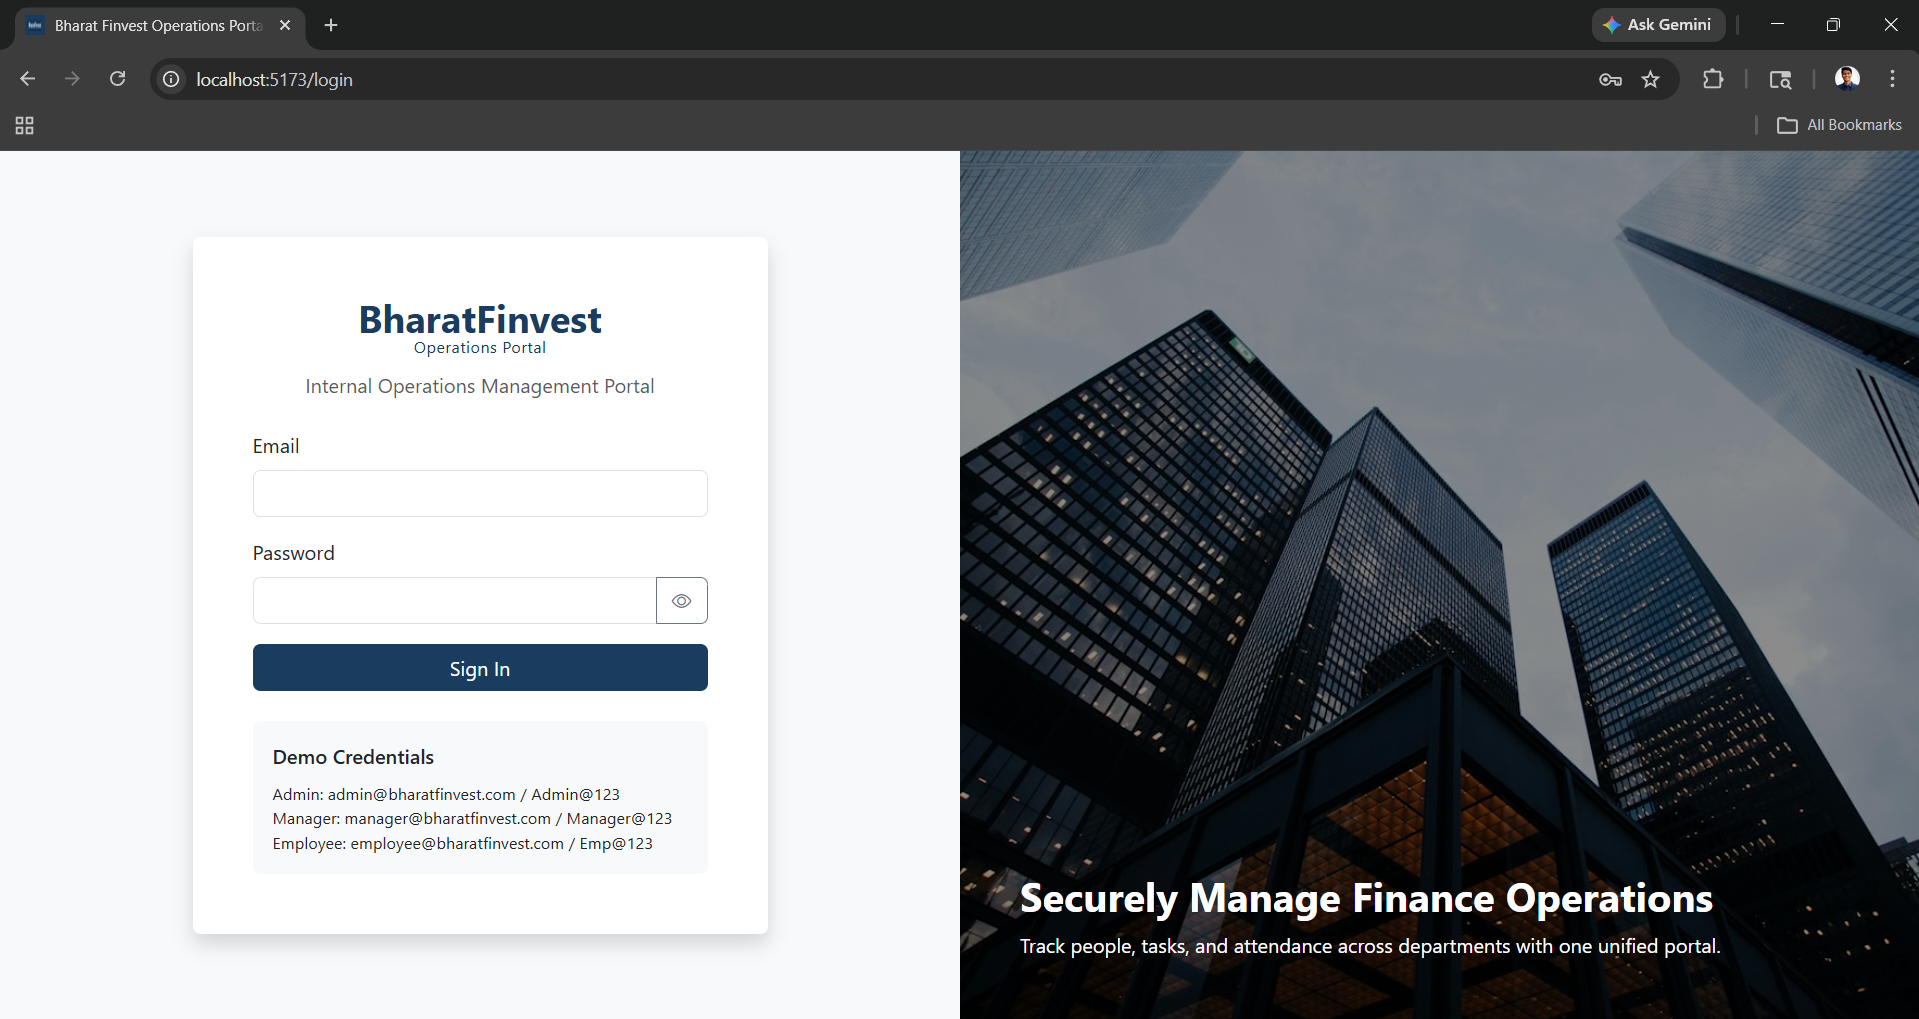
\includegraphics[width=0.95\textwidth]{images/login.png}
\caption{Login Screen}
\end{figure}
\clearpage

\section{Dashboard Screen}
\begin{figure}[H]
\centering
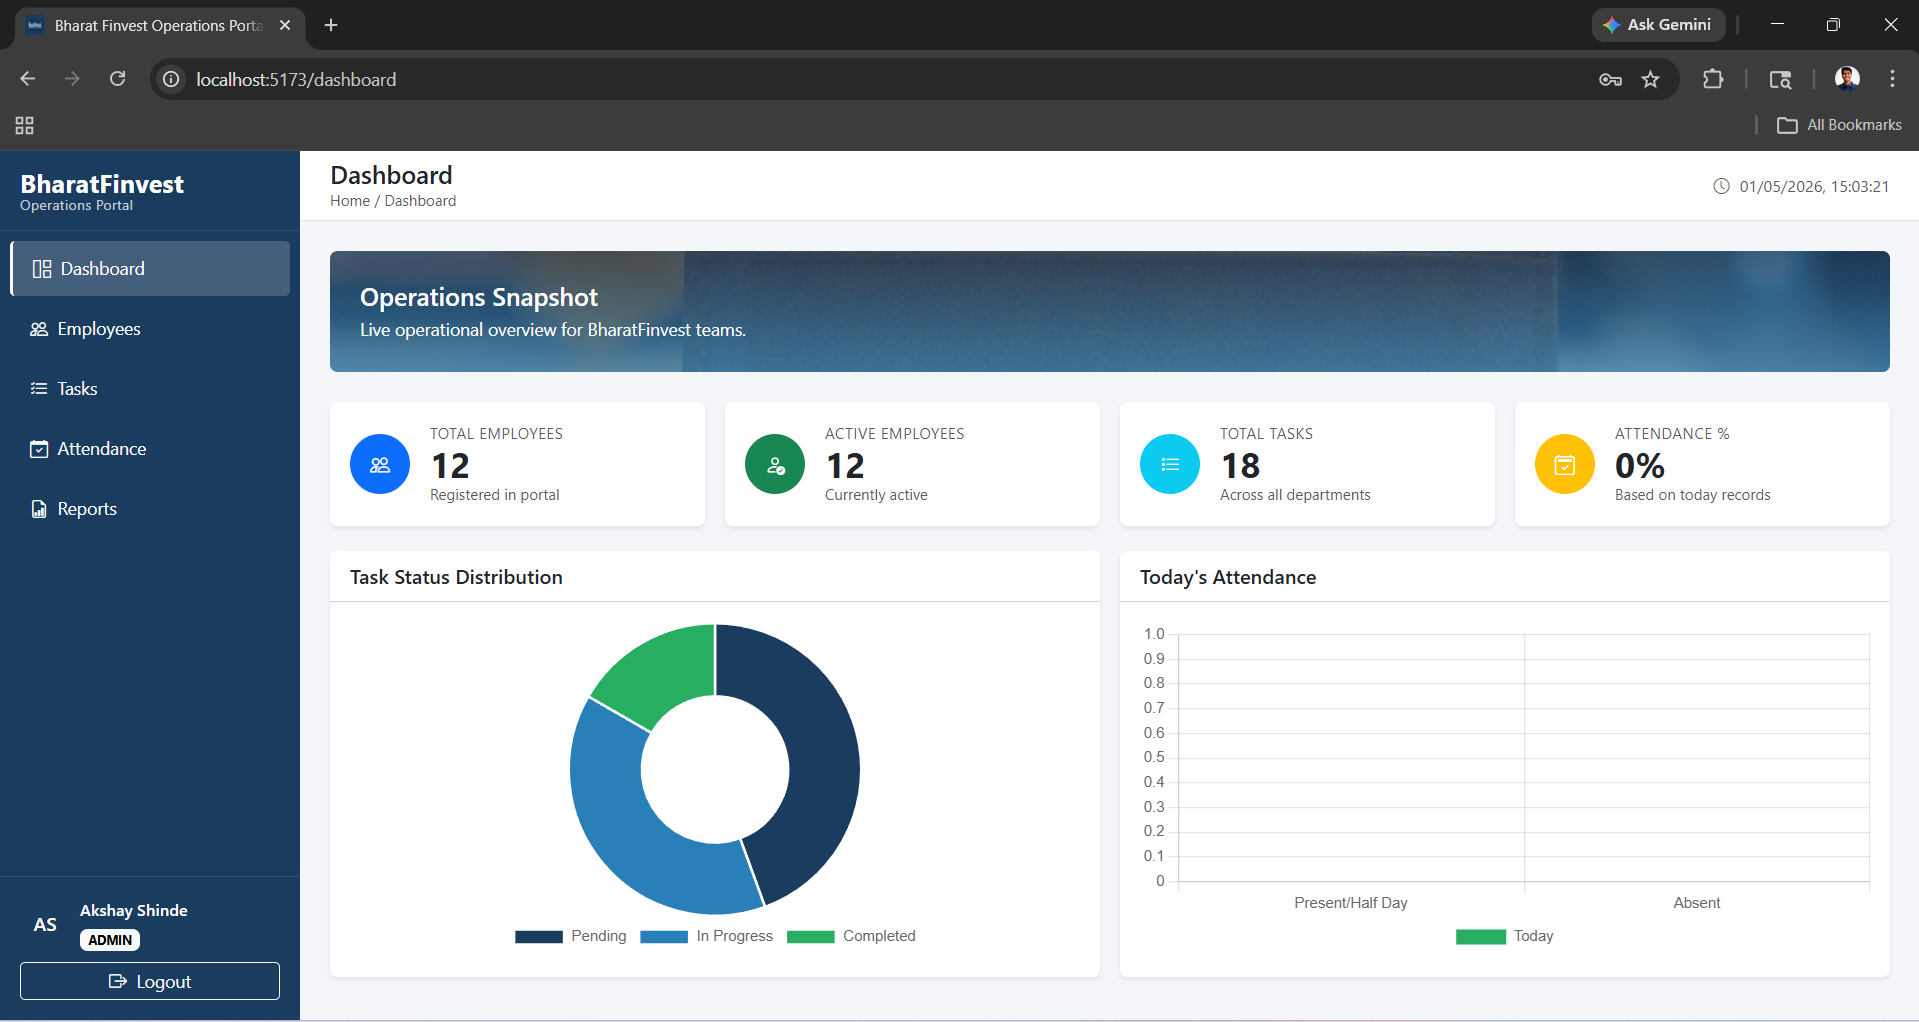
\includegraphics[width=0.95\textwidth]{images/dashboard.png}
\caption{Dashboard Screen}
\end{figure}
\clearpage

\section{Employees Screen}
\begin{figure}[H]
\centering
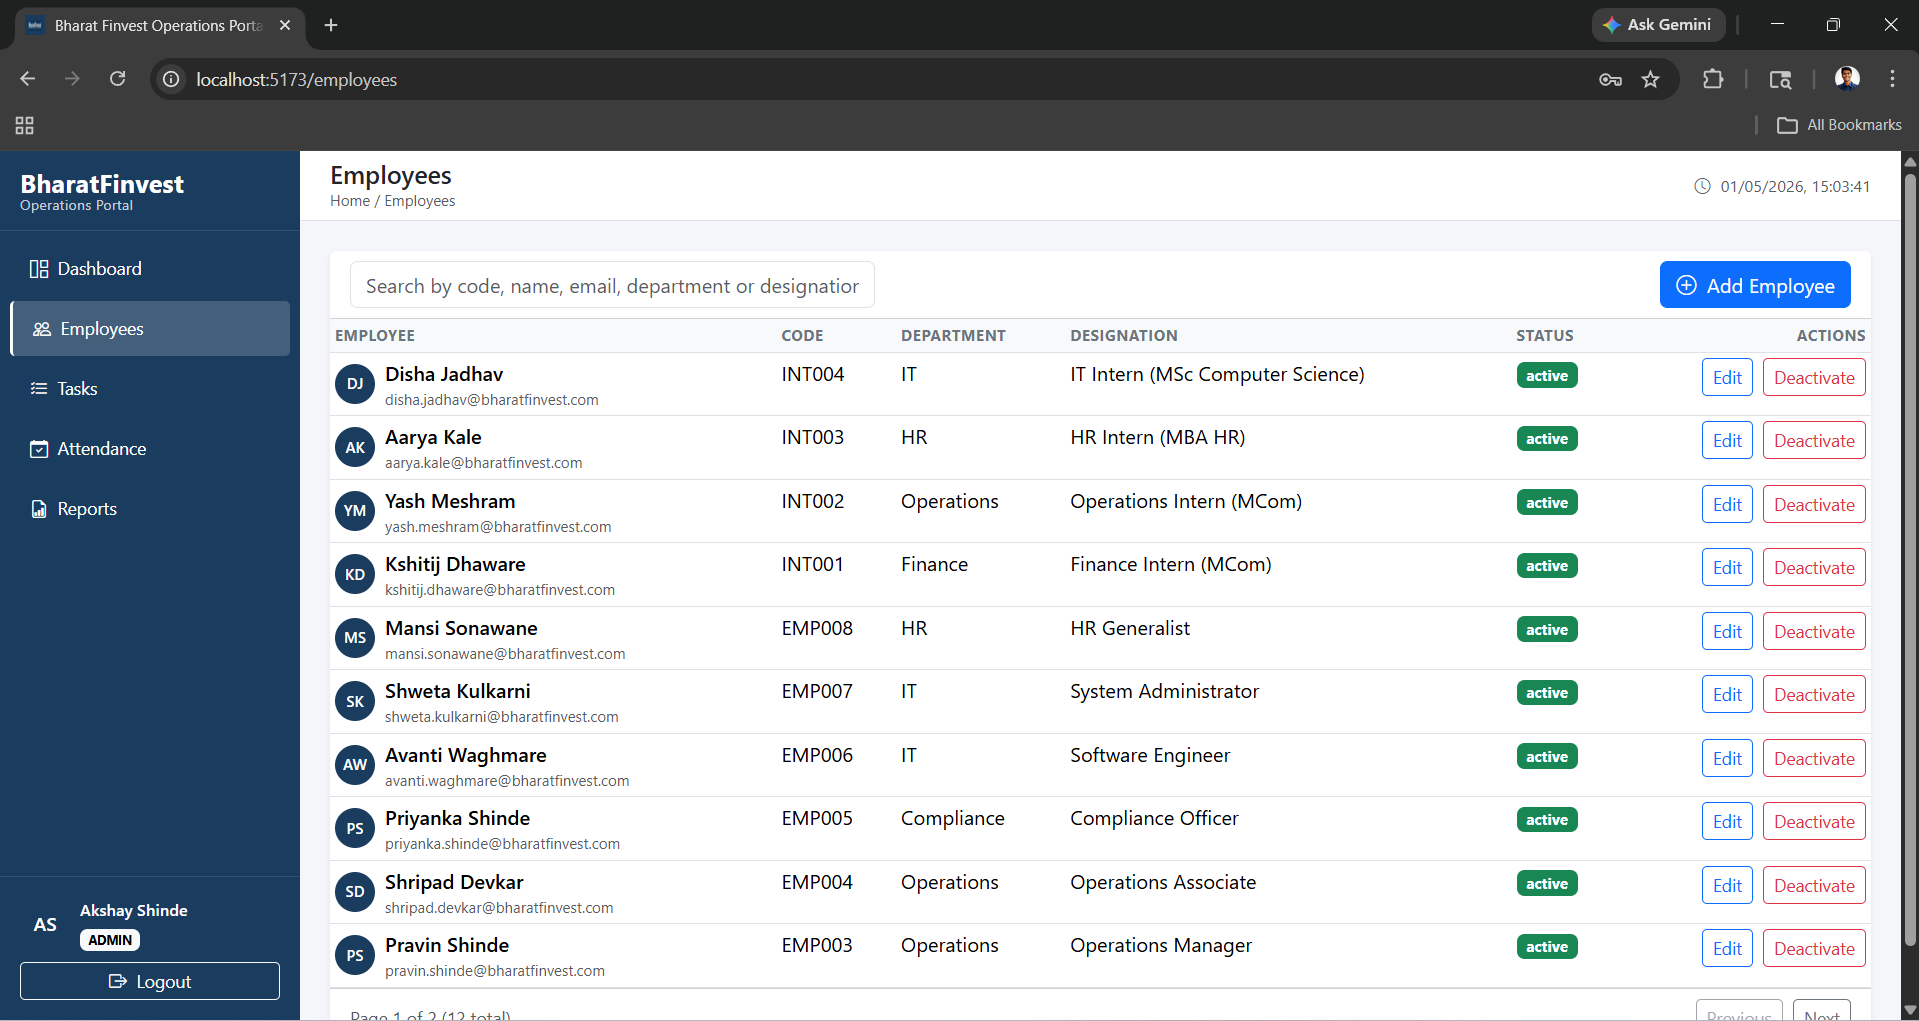
\includegraphics[width=0.95\textwidth]{images/employees.png}
\caption{Employees Screen}
\end{figure}
\clearpage

\section{Tasks Screen}
\begin{figure}[H]
\centering
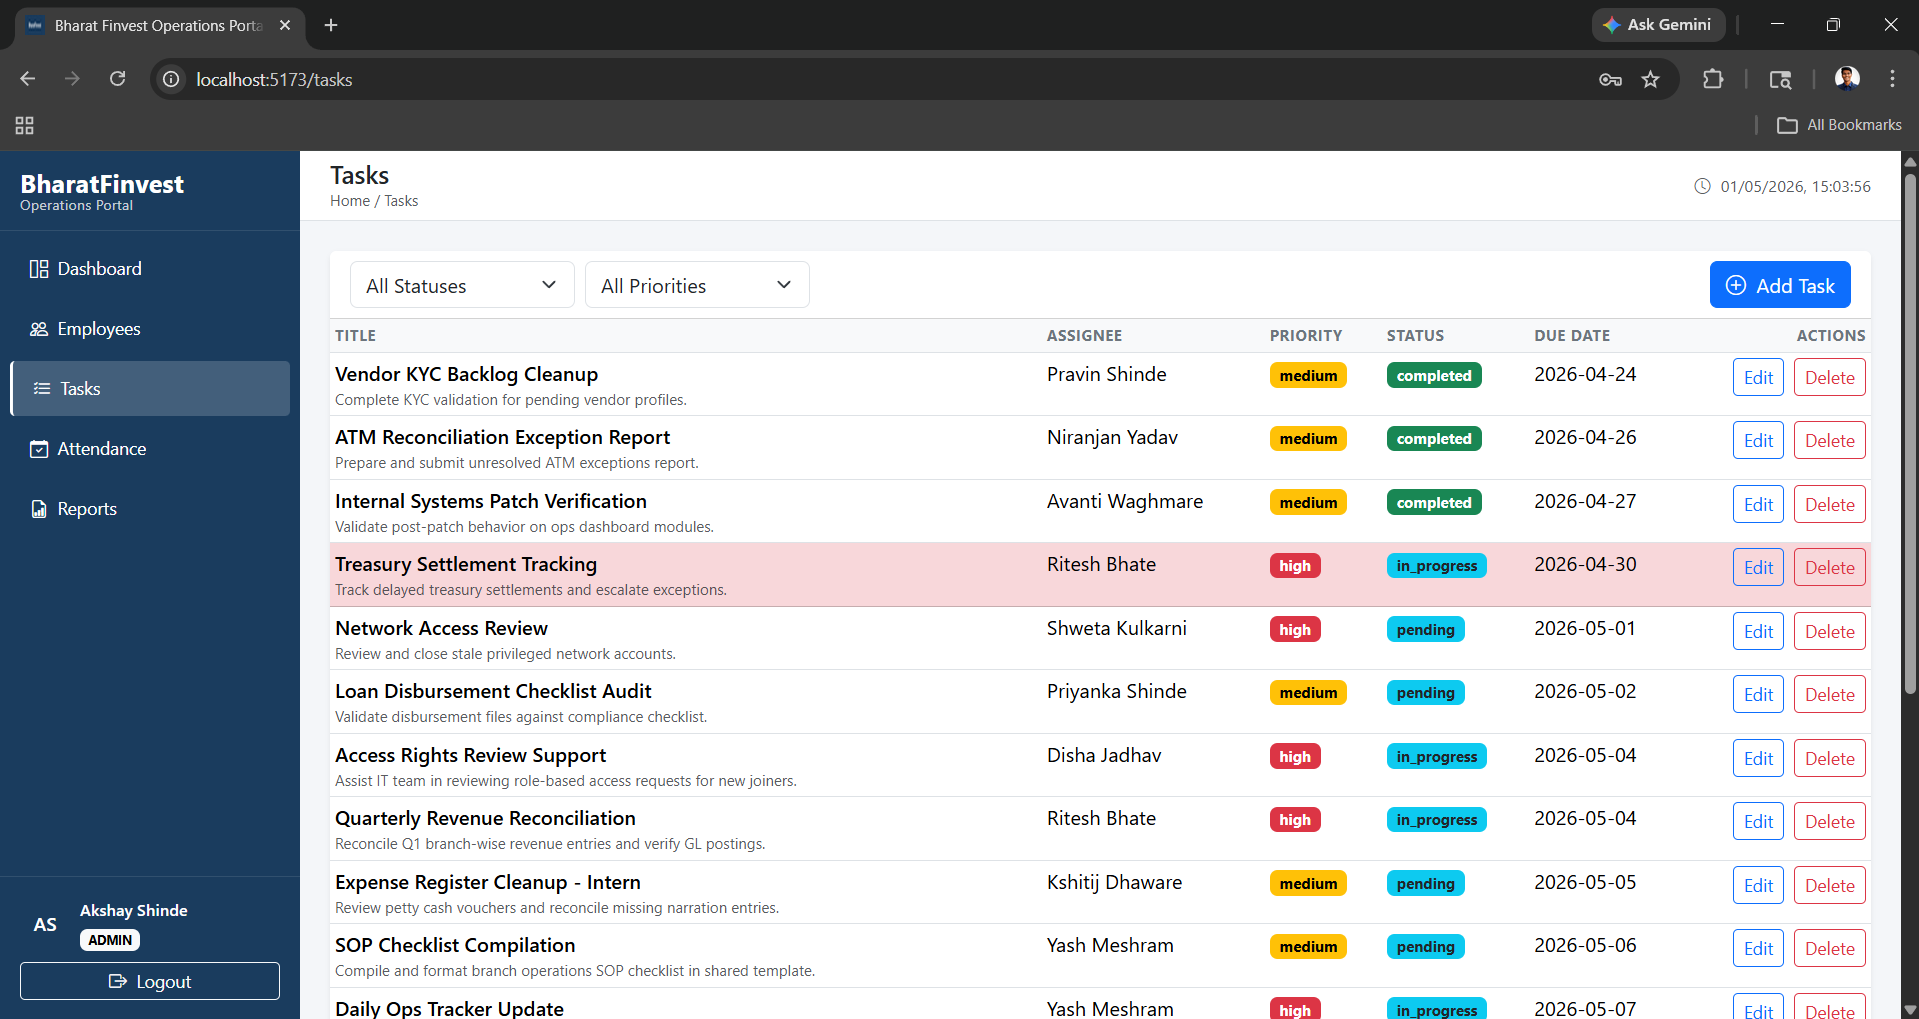
\includegraphics[width=0.95\textwidth]{images/tasks.png}
\caption{Tasks Screen}
\end{figure}
\clearpage

\section{Attendance Screen}
\begin{figure}[H]
\centering
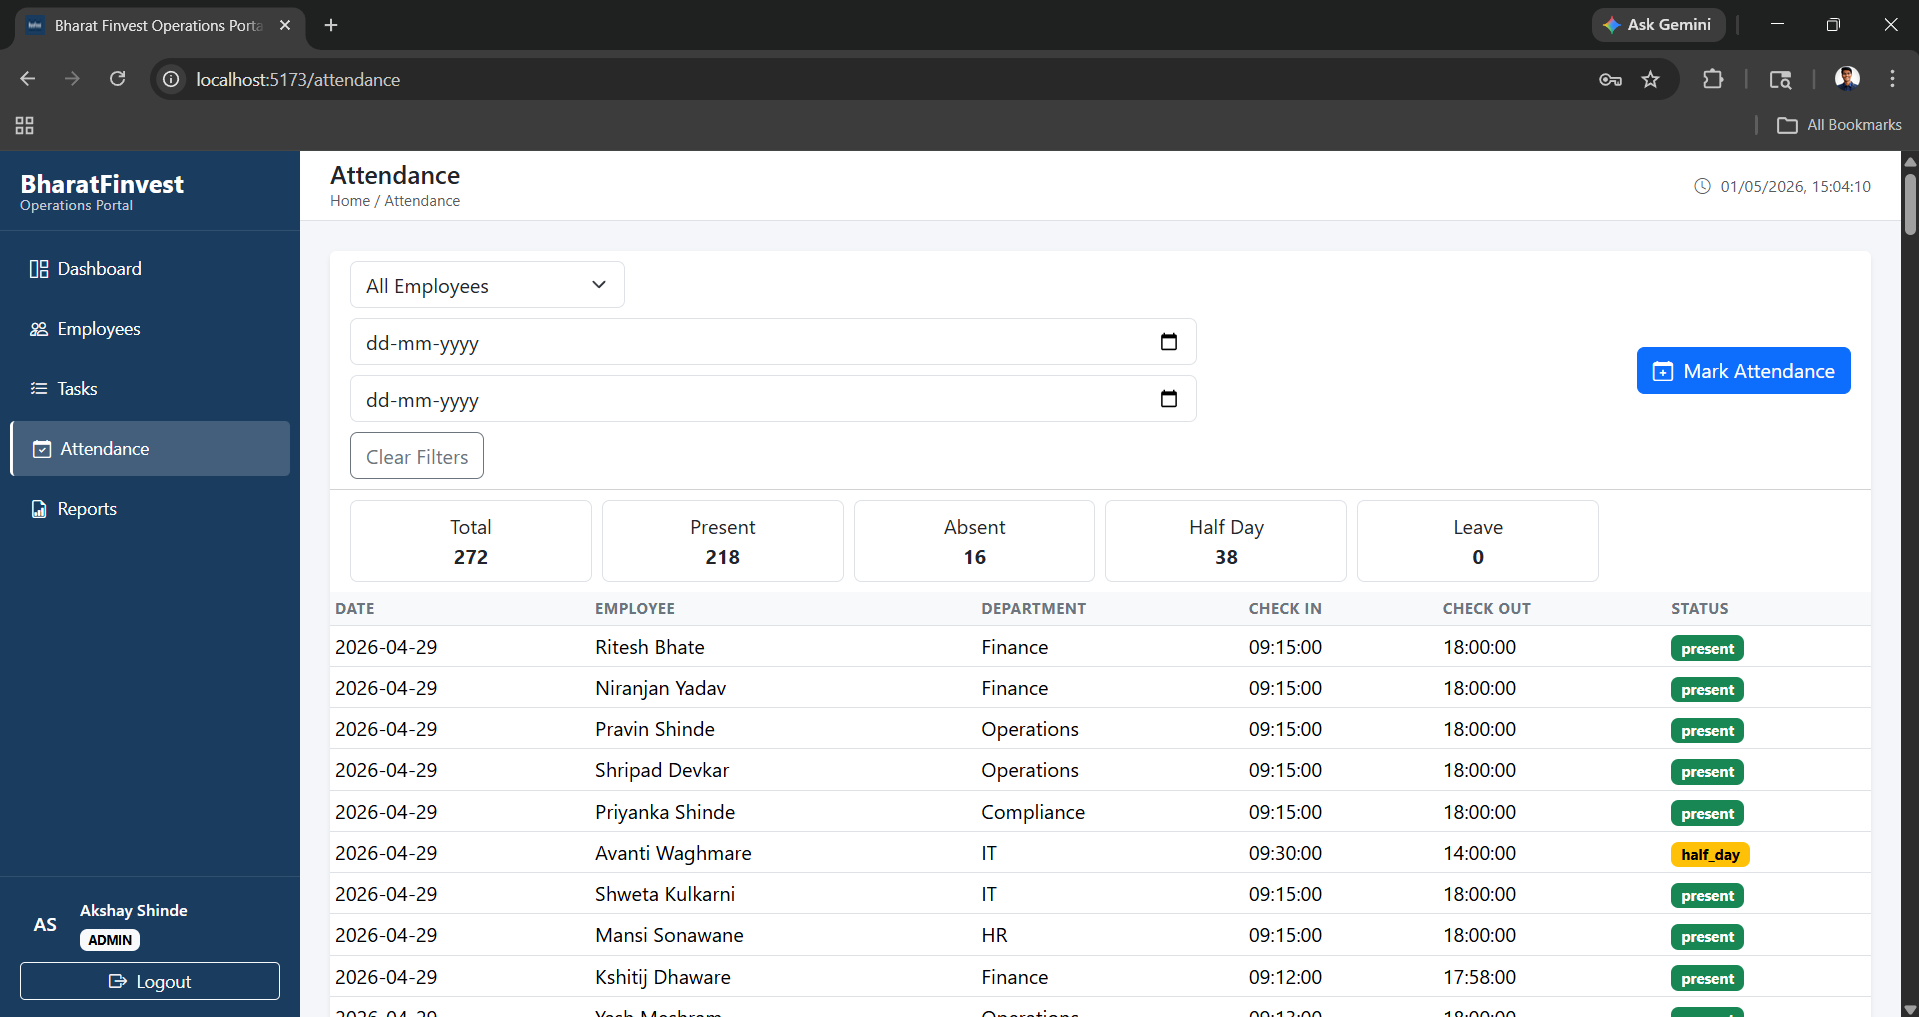
\includegraphics[width=0.95\textwidth]{images/attendance.png}
\caption{Attendance Screen}
\end{figure}
\clearpage

\section{Reports Screen}
\begin{figure}[H]
\centering
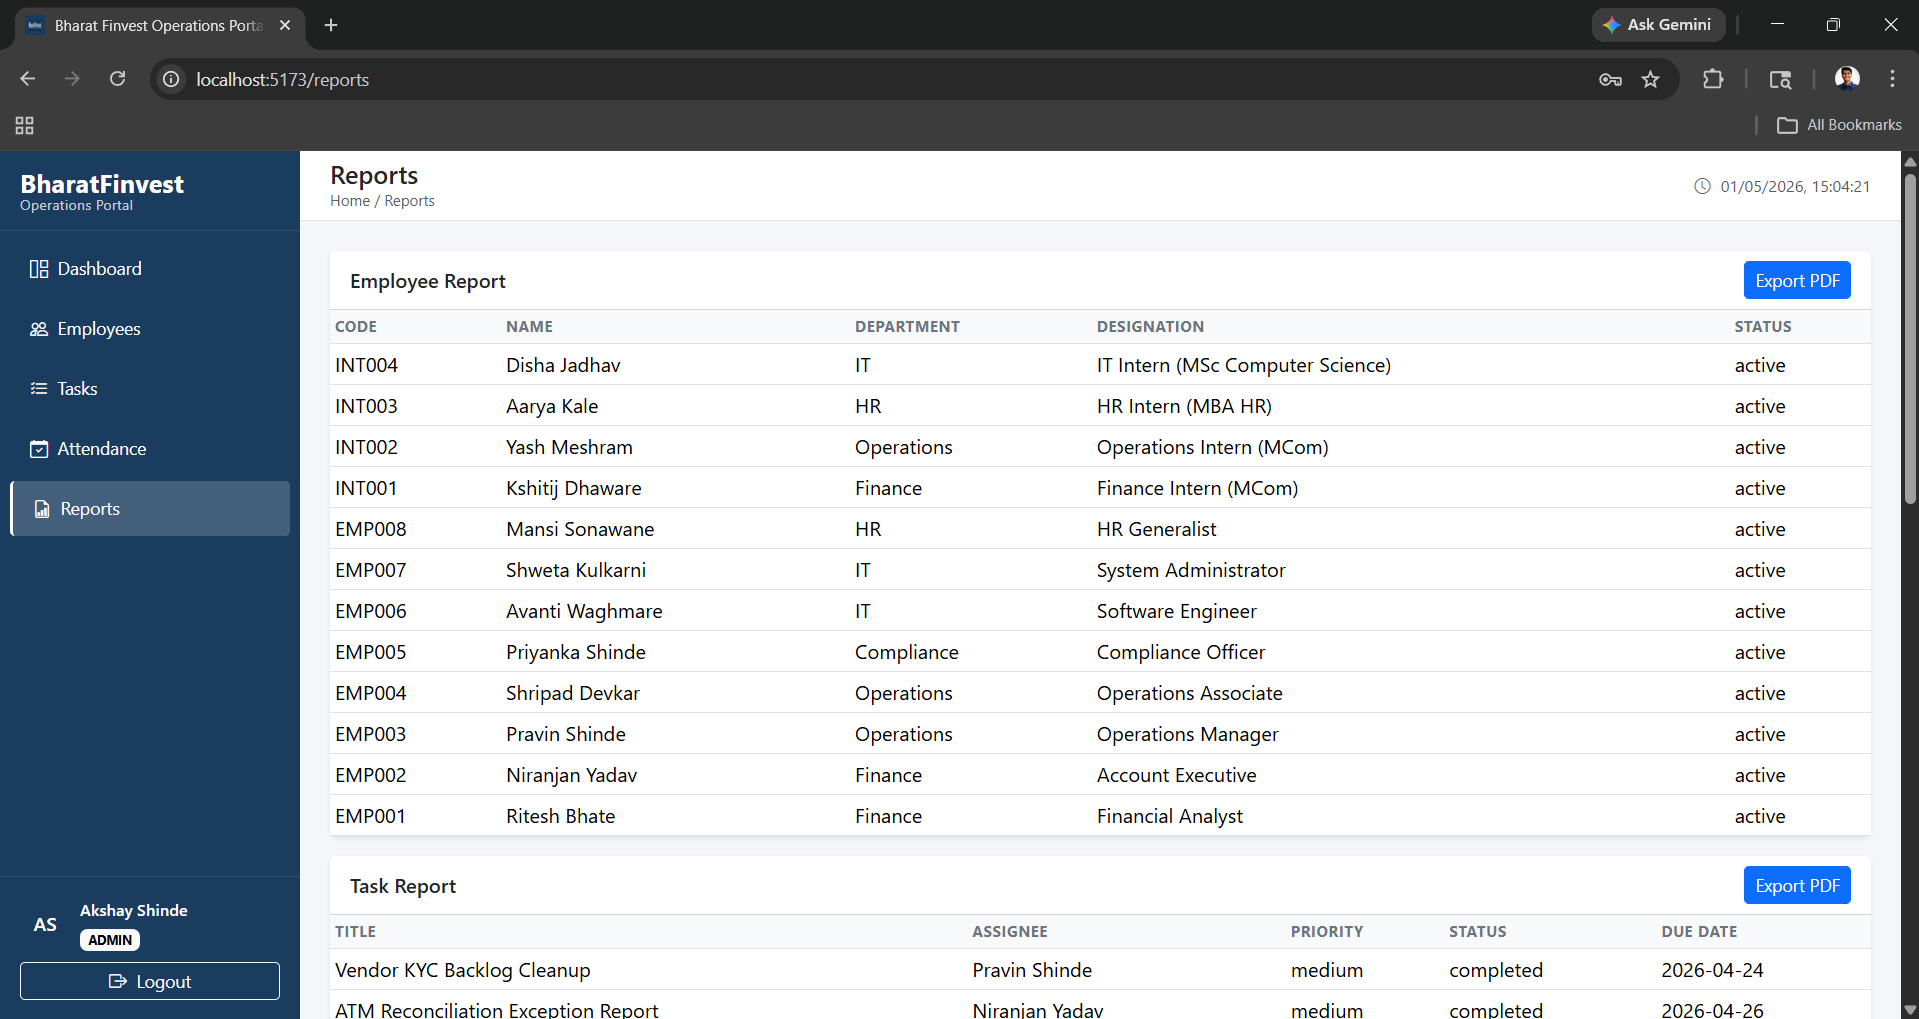
\includegraphics[width=0.95\textwidth]{images/reports.png}
\caption{Reports Screen}
\end{figure}

\chapter{API Design}

All APIs are exposed by the backend under the \texttt{/api} prefix and return JSON responses.

\setlength{\LTleft}{0pt}
\setlength{\LTright}{0pt}
\setlength{\tabcolsep}{4pt}
\renewcommand{\arraystretch}{1.18}
\newcolumntype{L}[1]{>{\raggedright\arraybackslash}p{#1}}
\small

\section{Authentication APIs}
\begin{longtable}{L{1.5cm}L{4.8cm}L{2.2cm}L{5.9cm}}
\toprule
\textbf{Method} & \textbf{Endpoint} & \textbf{Access} & \textbf{Purpose} \\
\midrule
\endhead
POST & \texttt{/api/auth/login} & Public & Validates email and password. On success returns \texttt{token} and \texttt{user}. \\
GET & \texttt{/api/auth/me} & Authenticated & Returns latest user profile from database for current JWT. \\
\bottomrule
\end{longtable}

\textbf{Login Request Example}
\begin{verbatim}
{
  "email": "admin@bharatfinvest.com",
  "password": "Admin@123"
}
\end{verbatim}

\textbf{Login Response Example}
\begin{verbatim}
{
  "token": "<jwt_token>",
  "user": {
    "id": 1,
    "name": "Akshay Shinde",
    "email": "admin@bharatfinvest.com",
    "role": "admin",
    "department": "Administration"
  }
}
\end{verbatim}

\section{Dashboard API}
\begin{longtable}{L{1.5cm}L{4.8cm}L{2.2cm}L{5.9cm}}
\toprule
\textbf{Method} & \textbf{Endpoint} & \textbf{Access} & \textbf{Purpose} \\
\midrule
\endhead
GET & \texttt{/api/dashboard/stats} & Authenticated & Returns employee counts, task stats, and today's attendance summary for dashboard widgets and charts. \\
\bottomrule
\end{longtable}

\section{Employee APIs}
\begin{longtable}{L{1.5cm}L{4.8cm}L{2.2cm}L{5.9cm}}
\toprule
\textbf{Method} & \textbf{Endpoint} & \textbf{Access} & \textbf{Purpose} \\
\midrule
\endhead
GET & \texttt{/api/employees} & Authenticated & Paginated and searchable list of employees (supports page, limit, search). \\
GET & \texttt{/api/employees/:id} & Authenticated & Employee detail with task count and attendance percentage. \\
POST & \texttt{/api/employees} & Admin, Manager & Creates employee record. \\
PUT & \texttt{/api/employees/:id} & Admin, Manager & Updates employee profile data or status. \\
DELETE & \texttt{/api/employees/:id} & Admin & Soft deactivates employee (status set to inactive). \\
\bottomrule
\end{longtable}

\section{Task APIs}
\begin{longtable}{L{1.5cm}L{4.8cm}L{2.2cm}L{5.9cm}}
\toprule
\textbf{Method} & \textbf{Endpoint} & \textbf{Access} & \textbf{Purpose} \\
\midrule
\endhead
GET & \texttt{/api/tasks} & Authenticated & Returns task list with optional filters: status, priority, assigned\_to. \\
GET & \texttt{/api/tasks/stats} & Authenticated & Returns aggregate task status counts. \\
GET & \texttt{/api/tasks/:id} & Authenticated & Returns one task with assignee and assigner names. \\
POST & \texttt{/api/tasks} & Admin, Manager & Creates a new task linked to employee and assigner user. \\
PUT & \texttt{/api/tasks/:id} & Admin, Manager & Updates task fields. \\
DELETE & \texttt{/api/tasks/:id} & Admin & Permanently deletes task record. \\
\bottomrule
\end{longtable}

\section{Attendance APIs}
\begin{longtable}{L{1.5cm}L{4.8cm}L{2.2cm}L{5.9cm}}
\toprule
\textbf{Method} & \textbf{Endpoint} & \textbf{Access} & \textbf{Purpose} \\
\midrule
\endhead
GET & \texttt{/api/attendance} & Authenticated & Returns attendance records with filters: employee\_id, from, and to. \\
POST & \texttt{/api/attendance} & Admin, Manager & Marks attendance for employee/date; duplicate entries are handled with HTTP 409 conflict response. \\
PUT & \texttt{/api/attendance/:id} & Admin, Manager & Updates an existing attendance row. \\
GET & \texttt{/api/attendance/summary} & Authenticated & Returns monthly summary per employee with attendance percentage. \\
\bottomrule
\end{longtable}

\section{Health API}
\begin{longtable}{L{1.5cm}L{4.8cm}L{2.2cm}L{5.9cm}}
\toprule
\textbf{Method} & \textbf{Endpoint} & \textbf{Access} & \textbf{Purpose} \\
\midrule
\endhead
GET & \texttt{/api/health} & Public & Performs \texttt{SELECT 1}; reports application and database health for monitoring. \\
\bottomrule
\end{longtable}
\normalsize

\section{API Error Strategy}
\begin{itemize}[leftmargin=1.3cm]
\item Validation failures return HTTP 400 with JSON message.
\item Unauthorized and forbidden access return HTTP 401 and 403 respectively.
\item Duplicate key or foreign-key conflicts return specific status codes (409 or 422).
\item Unknown routes return HTTP 404 JSON via fallback middleware.
\item Unhandled server errors are standardized through global error handler.
\end{itemize}


\chapter{Security Implementation}

\section{Authentication Security}
\begin{itemize}[leftmargin=1.3cm]
\item User authentication uses JSON Web Token (JWT).
\item Login credentials are validated against hashed passwords in database.
\item Access token is required in \texttt{Authorization: Bearer <token>} header for protected APIs.
\item Backend middleware verifies token signature and expiration.
\end{itemize}

\section{Password Security with bcrypt}
\begin{itemize}[leftmargin=1.3cm]
\item Passwords are not stored in plaintext.
\item \texttt{bcrypt.compare()} is used during login to verify entered password against stored hash.
\item Seeded demo accounts include pre-generated bcrypt hashes.
\end{itemize}

\section{Role-Based Access Control}
\begin{itemize}[leftmargin=1.3cm]
\item \texttt{authMiddleware} authenticates request and populates \texttt{req.user}.
\item \texttt{allowRoles(...)} middleware restricts access by role.
\item Examples:
  \begin{itemize}[leftmargin=1.1cm]
  \item Employee deactivation and task deletion are admin-only.
  \item Create/update employee/task/attendance are admin/manager-level actions.
  \end{itemize}
\end{itemize}

\section{Database and Query Security}
\begin{itemize}[leftmargin=1.3cm]
\item Backend uses \texttt{mysql2/promise} with parameterized queries.
\item Query placeholders prevent SQL injection on dynamic inputs.
\item Constraints such as unique keys and foreign keys protect data integrity.
\end{itemize}

\section{Client-Side Session Handling}
\begin{itemize}[leftmargin=1.3cm]
\item Token and user data are stored in localStorage for session continuity.
\item On app load, \texttt{/api/auth/me} refreshes user profile from backend.
\item Axios interceptor handles 401 responses by clearing local state and redirecting to login.
\end{itemize}

\section{Operational Security Hygiene}
\begin{itemize}[leftmargin=1.3cm]
\item \texttt{.env} is excluded from version control.
\item \texttt{node\_modules} and SQL backup dumps are ignored in \texttt{.gitignore}.
\item CORS origin is explicitly set to \texttt{http://localhost:5173} in backend app configuration.
\end{itemize}

\chapter{DevOps Implementation}

\section{Dockerization Strategy}
The project is container-ready with separate services for MySQL, backend API, and frontend web server.

\begin{itemize}[leftmargin=1.3cm]
\item \texttt{backend/Dockerfile}: builds Node.js backend image and runs \texttt{server.js} on port 5000.
\item \texttt{frontend/Dockerfile}: builds React app and serves static output with Nginx.
\item \texttt{frontend/nginx.conf}: handles SPA fallback routing and proxies \texttt{/api} requests to backend service.
\end{itemize}

\section{Docker Compose Orchestration}
\texttt{docker-compose.yml} defines three services:
\begin{itemize}[leftmargin=1.3cm]
\item \textbf{mysql}: MySQL 8 container with initialization from \texttt{database/} scripts.
\item \textbf{backend}: Depends on healthy MySQL and exposes port 5000.
\item \textbf{frontend}: Depends on healthy backend and exposes port 80.
\end{itemize}

\section{Health Checks}
\begin{itemize}[leftmargin=1.3cm]
\item MySQL health check uses \texttt{mysqladmin ping}.
\item Backend health check calls \texttt{GET /api/health} from inside container.
\item Health endpoint runs \texttt{SELECT 1} query to confirm database connectivity.
\item If database check fails, endpoint returns HTTP 503 with \texttt{database: disconnected}.
\end{itemize}

\section{GitHub Actions CI Pipeline}
\texttt{.github/workflows/ci.yml} automatically runs on push and pull request.

\begin{itemize}[leftmargin=1.3cm]
\item Sets up Node.js 20.
\item Installs backend dependencies using \texttt{npm install}.
\item Verifies backend app import with \texttt{node -e "require('./backend/src/app')"}-style check.
\item Installs frontend dependencies and executes \texttt{npm run build}.
\end{itemize}

This pipeline quickly catches import errors and frontend build failures before deployment.

\section{Windows Automation Scripts}
\subsection*{1. One-click startup script}
\texttt{start-project.bat}:
\begin{itemize}[leftmargin=1.3cm]
\item Detects Node/npm availability.
\item Installs backend/frontend dependencies only if \texttt{node\_modules} is missing.
\item Starts backend and frontend in separate CMD windows.
\item Opens browser at \texttt{http://localhost:5173}.
\end{itemize}

\subsection*{2. Backup script}
\texttt{scripts/backup-db.bat}:
\begin{itemize}[leftmargin=1.3cm]
\item Uses full-path \texttt{mysqldump.exe}.
\item Creates \texttt{backups/} if missing.
\item Produces timestamped SQL dump file for \texttt{bharat\_finvest\_ops}.
\end{itemize}

\subsection*{3. Restore script}
\texttt{scripts/restore-db.bat}:
\begin{itemize}[leftmargin=1.3cm]
\item Accepts drag/drop backup file path from user.
\item Uses full-path \texttt{mysql.exe} to restore selected dump into target database.
\end{itemize}

\section{Environment-based Configuration}
Backend configuration uses environment variables from \texttt{backend/.env}:
\texttt{DB\_HOST}, \texttt{DB\_PORT}, \texttt{DB\_USER}, \texttt{DB\_PASSWORD}, \texttt{DB\_NAME}, \texttt{JWT\_SECRET}, \texttt{JWT\_EXPIRES\_IN}, and \texttt{PORT}.

This design supports local execution, Docker execution, and future production deployment with minimal changes.

\chapter{Testing Strategies}

The project validation was performed using a layered testing strategy to improve reliability and demo safety.

\section{Unit-level Validation}
Full formal unit test suites are not yet introduced with Jest/Mocha; however, core logic was validated at function level through controlled API requests and deterministic input scenarios.

\textbf{Examples:}
\begin{itemize}[leftmargin=1.3cm]
\item Payload validation for employee/task/attendance controllers.
\item Duplicate handling paths (attendance duplicate entry, employee duplicate keys).
\item JWT middleware accept/reject flows.
\end{itemize}

\section{Integration Testing}
Integration testing focused on API-to-database behavior.
\begin{itemize}[leftmargin=1.3cm]
\item CRUD flows were tested against real MySQL schema.
\item Foreign key constraints were verified through valid/invalid references.
\item Dashboard and summary APIs were validated for aggregated SQL output.
\end{itemize}

\section{System Testing}
System testing validated end-to-end behavior from browser to database.
\begin{itemize}[leftmargin=1.3cm]
\item Login and protected routing.
\item Employee, task, and attendance operation sequence.
\item PDF generation in reports page.
\item Logout and stale session fallback behavior.
\end{itemize}

\section{UI/UX Testing}
UI testing was executed with focus on visible controls and modal flows.
\begin{itemize}[leftmargin=1.3cm]
\item All actionable buttons were verified for expected behavior.
\item Required fields and form validation states were checked.
\item Success/error banners were verified after API responses.
\item Loading states and disabled buttons were verified during requests.
\end{itemize}

\section{Build and Runtime Verification}
\begin{itemize}[leftmargin=1.3cm]
\item Backend import verification: \texttt{node -e "require('./src/app')"}
\item Frontend production build verification: \texttt{npm run build}
\item Health endpoint verification: \texttt{GET /api/health}
\item CI build verification in GitHub Actions pipeline.
\end{itemize}

\section{Regression Safety}
Changes for branding, avatar logic, and DevOps enhancements were validated to ensure no break in existing core modules:
\begin{itemize}[leftmargin=1.3cm]
\item Login module remains functional.
\item Dashboard metrics continue loading.
\item CRUD operations remain stable.
\item PDF exports continue generating non-empty documents.
\end{itemize}

\chapter{Test Cases}

\setlength{\LTleft}{0pt}
\setlength{\LTright}{0pt}
\setlength{\tabcolsep}{3pt}
\renewcommand{\arraystretch}{1.16}
\newcolumntype{T}[1]{>{\raggedright\arraybackslash}p{#1}}
\footnotesize

\begin{longtable}{T{0.9cm}T{2.4cm}T{3.0cm}T{5.0cm}T{1.7cm}}
\toprule
\textbf{ID} & \textbf{Test Case} & \textbf{Input / Action} & \textbf{Expected Result} & \textbf{Status} \\
\midrule
\endhead
TC01 & Login success & Valid admin credentials & Redirect to dashboard with active session and sidebar user details. & Pass \\
TC02 & Login failure & Invalid password & Error alert shown for invalid credentials. & Pass \\
TC03 & Auth refresh & Existing JWT, app reload & \texttt{/api/auth/me} refreshes user and updates localStorage state. & Pass \\
TC04 & Employee list load & Open Employees page & Paginated data displayed with search and avatar initials. & Pass \\
TC05 & Add employee & Submit valid Add Employee form & New employee created, success banner shown, table refreshed. & Pass \\
TC06 & Edit employee & Update existing employee details & Employee updated, modal closes after success, table refreshed. & Pass \\
TC07 & Deactivate employee & Admin clicks Deactivate and confirms & Employee status changes to inactive with success banner. & Pass \\
TC08 & Task list filter & Apply status and priority filters & Task table shows matching filtered records only. & Pass \\
TC09 & Add task & Submit valid task form with assignee & Task created and visible in refreshed list. & Pass \\
TC10 & Edit task & Update task status or due date & Task updated while preserving relational links. & Pass \\
TC11 & Delete task & Admin confirms task deletion & Task removed from database and UI list. & Pass \\
TC12 & Mark attendance & Submit employee/date/status in modal & Attendance entry inserted and table refreshed. & Pass \\
TC13 & Duplicate attendance guard & Mark same employee/date twice & API returns conflict; UI displays error in modal. & Pass \\
TC14 & Attendance filters & Filter by employee and date range & Table updates with matching records. & Pass \\
TC15 & Employee PDF export & Click Export PDF in Reports page & Downloaded PDF contains employee rows and header. & Pass \\
TC16 & Task PDF export & Click Export PDF in Reports page & Downloaded PDF contains task data with timestamp. & Pass \\
TC17 & Attendance PDF export & Click Export PDF in Reports page & Downloaded PDF contains attendance summary table. & Pass \\
TC18 & Logout flow & Click sidebar logout button & Token and user are removed; route redirects to login. & Pass \\
TC19 & Health API success & GET \texttt{/api/health} with DB available & JSON response shows status OK and database connected. & Pass \\
TC20 & Unauthorized route & Call protected API without token & HTTP 401 JSON error response returned. & Pass \\
\bottomrule
\end{longtable}
\normalsize

\section*{Notes on Evidence Collection}
\begin{itemize}[leftmargin=1.3cm]
\item API responses were verified through browser-driven requests and backend logs.
\item Frontend behavior was verified with modal actions, alerts, and table refresh checks.
\item Build and import checks were also validated through command-line verification and CI workflow.
\end{itemize}

\chapter{Limitations}

Although the application is stable for academic demonstration and prototype usage, the following limitations are currently present:

\begin{itemize}[leftmargin=1.3cm]
\item Role policy is practical for demo but can be expanded with finer permission granularity (module-level/field-level controls).
\item Automated unit and integration test suites are not fully formalized with a dedicated testing framework.
\item Audit trail for all data changes (who changed what and when) is not yet implemented as a separate module.
\item Notification workflows (email/SMS reminders for overdue tasks or missing attendance) are not integrated.
\item Large-scale pagination and server-side report batching are basic; advanced performance tuning can be introduced for high-volume production traffic.
\item Deployment is currently local/container-ready; cloud production deployment pipeline is not yet configured.
\item Mobile-first UX optimization can be enhanced for long operational tables on very small screens.
\end{itemize}

\chapter{Future Scope}

The following enhancements are proposed for the next phase:

\begin{enumerate}[leftmargin=1.3cm]
\item \textbf{Email Notifications:} Automated emails for task assignment, due reminders, and attendance irregularities.
\item \textbf{SMS Alerts:} Optional SMS notifications for urgent operational actions.
\item \textbf{Payroll Integration:} Connect attendance and role data with payroll calculations.
\item \textbf{Leave Management Module:} Add leave request, approval workflow, and leave balance tracking.
\item \textbf{Cloud Deployment:} Deploy backend/frontend/database to cloud infrastructure for wider usage.
\item \textbf{Jenkins Pipeline:} Add an enterprise CI/CD option alongside GitHub Actions.
\item \textbf{Advanced Analytics:} Department productivity trends, SLA tracking, and predictive summaries.
\item \textbf{Audit Logs:} Immutable activity log for compliance and security review.
\item \textbf{Document Management:} Upload and attach operational documents to tasks or employee profiles.
\item \textbf{Role Customization:} Configurable permissions with policy templates per business unit.
\end{enumerate}

These additions would transition the current prototype into a more comprehensive enterprise operations platform.

\chapter{Conclusion}

The \textbf{Bharat Finvest Internal Operations Management System} was successfully designed and implemented as a full-stack industrial training project for M.Sc. (Computer Science) Part II, Sem IV.

This project was developed during industrial training at \textbf{Nityashree Infosystems Pvt. Ltd.} as a client-style internal operations management system for \textbf{Bharat Finvest}.

The final system demonstrates:
\begin{itemize}[leftmargin=1.3cm]
\item Secure login with JWT and role-aware authorization.
\item Practical employee, task, and attendance workflow management.
\item Dashboard-level operational visibility through computed metrics and charts.
\item Exportable PDF reports for documentation and review needs.
\item Production-oriented operational support through Docker, health checks, CI, and backup/restore scripts.
\end{itemize}

The project aligns with both academic objectives and real-world operational requirements by combining software engineering principles, relational database design, API development, and DevOps practices in one coherent solution.

Hence, the project is suitable for final presentation, academic assessment, and further extension toward production readiness. This report does not claim official production deployment within Bharat Finvest.

\chapter{Bibliography \& References}

\begin{enumerate}[leftmargin=1.3cm]
\item Bharat Finvest Ops project repository: \url{https://github.com/tejasskamble/bharat-finvest-ops-system}
\item Project source files inspected directly from local repository (backend, frontend, database, and DevOps files).
\item Reference format document: \texttt{MSC IT Project report Cover Page(1).docx}
\item Certificate format reference: \texttt{MSC IT certificates.pdf}
\item Sample report structure reference: \texttt{Final\_It\_Report.pdf}
\item Internal evaluation guideline reference: \texttt{IT Project Internal Evalution guideline.pdf}
\item React documentation: \url{https://react.dev/}
\item Vite documentation: \url{https://vitejs.dev/}
\item Express documentation: \url{https://expressjs.com/}
\item MySQL 8 documentation: \url{https://dev.mysql.com/doc/}
\item JWT introduction: \url{https://jwt.io/introduction}
\item bcrypt package documentation: \url{https://www.npmjs.com/package/bcrypt}
\item Docker documentation: \url{https://docs.docker.com/}
\item GitHub Actions documentation: \url{https://docs.github.com/actions}
\item jsPDF documentation: \url{https://github.com/parallax/jsPDF}
\end{enumerate}

\chapter{Appendix}

\section{A. Training and Client Context}
\begin{itemize}[leftmargin=1.3cm]
\item Training Organization: \textbf{Nityashree Infosystems Pvt. Ltd.}
\item Client / Project Domain Organization: \textbf{Bharat Finvest}
\item Project Title: \textbf{Bharat Finvest Internal Operations Management System}
\end{itemize}

\section{B. GitHub Repository}
\url{https://github.com/tejasskamble/bharat-finvest-ops-system}

\section{C. Demo Credentials}
\begin{table}[H]
\centering
\small
\setlength{\tabcolsep}{4pt}
\begin{tabular}{p{2.5cm}p{6.0cm}p{2.5cm}}
\toprule
\textbf{Role} & \textbf{Email} & \textbf{Password} \\
\midrule
Admin & \texttt{admin@bharatfinvest.com} & \texttt{Admin@123} \\
Manager & \texttt{manager@bharatfinvest.com} & \texttt{Manager@123} \\
Employee & \texttt{employee@bharatfinvest.com} & \texttt{Emp@123} \\
\bottomrule
\end{tabular}
\end{table}
\normalsize

\section{D. Employee and Intern Seed Dataset}
\begin{itemize}[leftmargin=1.3cm]
\item Ritesh Bhate
\item Niranjan Yadav
\item Pravin Shinde
\item Shripad Devkar
\item Priyanka Shinde
\item Avanti Waghmare
\item Shweta Kulkarni
\item Mansi Sonawane
\item Kshitij Dhaware
\item Yash Meshram
\item Aarya Kale
\item Disha Jadhav
\end{itemize}

\section{E. Essential Commands}
\subsection*{1. Database Import (Windows CMD)}
\begin{verbatim}
mysql -u root -p < database\schema.sql
mysql -u root -p bharat_finvest_ops < database\seed.sql
\end{verbatim}
\textit{Note: If mysql is not in PATH, use the full executable path of mysql.exe.}

\subsection*{2. Backend Run}
\begin{verbatim}
cd backend
npm install
npm run dev
\end{verbatim}

\subsection*{3. Frontend Run}
\begin{verbatim}
cd frontend
npm install
npm run dev
\end{verbatim}

\subsection*{4. One-Click Run}
\begin{verbatim}
start-project.bat
\end{verbatim}

\subsection*{5. Health Check}
\begin{verbatim}
http://localhost:5000/api/health
\end{verbatim}

\subsection*{6. Docker Commands}
\begin{verbatim}
docker-compose up --build
docker-compose down
\end{verbatim}

\subsection*{7. Backup and Restore}
\begin{verbatim}
scripts\backup-db.bat
scripts\restore-db.bat
\end{verbatim}

\section{F. Final QA Checklist Reference}
\begin{itemize}[leftmargin=1.3cm]
\item Login tested
\item Dashboard tested
\item Employee CRUD tested
\item Task CRUD tested
\item Attendance tested
\item Reports PDF tested
\item Logout tested
\item Health API tested
\end{itemize}


\end{document}



